%%%%%%%%%%%%%%%%%%%%%%%%%%%%%%%%%%%%%%%%%%%%%%%%%%%%%%%%%%%%%%%%%%%%%%%%
%                                                                      %
% LaTeX, FIIW thesis template                                          %
% 
% Voor Nederlandse versie gebruik volgende lijnen code: 15,46,79,124   %
% For English Version use the following lines of code: 16,47,80,125    %
%%%%%%%%%%%%%%%%%%%%%%%%%%%%%%%%%%%%%%%%%%%%%%%%%%%%%%%%%%%%%%%%%%%%%%%%
\documentclass[11pt,a4paper]{report}
%% For english version
% Indien je je thesis recto-verso wil afdrukken gebruik je onderstaande opties i.p.v. bovenstaande
%\documentclass[11pt,a4paper,twoside,openright]{report}

\usepackage[a4paper,left=3.5cm, right=2.5cm, top=3.5cm, bottom=3.5cm]{geometry}

\usepackage[dutch]{babel}
\usepackage{graphicx}     % om niet ascii karakters rechtstreeks te kunnen inputten
\usepackage[utf8]{inputenc}            % commentarieer deze regel uit als je utf8 encoded files gebruikt in plaats van latin1
\usepackage[square, numbers]{natbib}    % Referentie opties [square, numbers] 
\usepackage{listings}             		% voor het weergeven van broncode
\usepackage{verbatim}					% weergeven van code, commando's, ...
\usepackage{hyperref}					% maak PDF van de thesis navigeerbaar
\usepackage{url}						% URL's invoegen in tekst met behulp van \url{http://}
\usepackage[small,bf,hang]{caption}     % om de captions wat te verbeteren
\usepackage[final]{pdfpages}            % gebruikt voor het invoegen van het artikel in pdf-formaat
\usepackage{pslatex}					% andere lettertype's dan de standaard types
\usepackage{lipsum}
\usepackage{sectsty}		            % aanpassen van de fonts van sections en chapters
\usepackage{subcaption}                 % subfiguren
%\usepackage[nottoc,numbib]{tocbibind}	% Bibliography mee in de ToC

\allsectionsfont{\sffamily}
\chapterfont{\raggedleft\sffamily}

\usepackage{float}                      % De optie H voor de plaatsing van figuren op de plaats waar je ze invoegt. bvb. \begin{figure}[H]
%\usepackage{longtable}					% tabellen die over meerdere pagina's gespreid worden
%\usepackage[times]{quotchap}           % indien je fancy hoofdstuktitels wil
%\usepackage[none]{hyphenat}
%\usepackage{latexsym}
%\usepackage{amsmath}
%\usepackage{amssymb}

% MFA: zet zoekpad voor figure
\graphicspath{{fig/}}

\usepackage{fiiw} % Voor de nedelandse versie

%door onderstaande regels in commentaar te zetten, of op false, kan je pagina's weglaten
%bijvoorbeeld het weglaten van een voorwoord, lijst met symbolen, ...
%%%%%%%%%%%%%%%%%%%%%%%%%%%%%%%%%%%%%%%%%%%%%%%%%%%%%%%%%%%%%%%%%%%%%%%%%%%%%%%%%%%%%%%%
%voorwoord toevoegen?

\acknowledgementspagetrue{}
\acknowledgements{voorwoord}			%.tex file met daarin het voorwoord

%samenvatting toevoegen
\summarypagetrue{}
\summary{samenvatting}					%.tex met daarin de samenvatting

%abstract toevoegen?
\abstractpagetrue{}
\abstracts{abstract}					%.tex file met daarin het abstract
%lijst van figuren toevoegen?
\listoffigurespagetrue{}
%lijst van tabellen toevoegen?
\listoftablespagetrue{}
%lijst van symbolen toevoegen?
% \listofsymbolspagetrue{}
\listofsymbols{symbolen}				%.tex file met daarin de lijst van symbolen
%lijst van afkortingen toevoegen?
\listofabbrevspagetrue{}
\listofabbrevs{afkortingen}				%.tex file met daarin de lijst van symbolen
\setlength{\parskip}{16pt}
%informatie over het eindwerk, de promotor, ...
%%%%%%%%%%%%%%%%%%%%%%%%%%%%%%%%%%%%%%%%%%%%%%%
\opleiding{Elektronica/ICT}
\afdeling{Optie Smart Applications}
\campus{gent} % Voor de Nederlandse versie van campus de nayer. Voor andere campussen gebuirk geel,gent,groept of brugge.

\title{Time Is Running Out}
\subtitle{Assessing Temporal Privacy of Privacy Zones in Fitness Tracking Social Networks}
% \author{naam student}
\forenameA{Wout}
\surnameA{Deleu}

\forenameB{}
\surnameB{}

\academicyear{2022 - 2023}

\promotorA[Promotor]{Prof. dr. ing. Stijn Volckaert}
\promotorB[Begeleiders]{Ing. Karel Dhondt, \\Ing. Alicia Andries \\Ing. Jonas Vinck}

\begin{document}
\selectlanguage{dutch}
\preface{}

%%%%%%%%%%%%%%%%%%%%%%%%%%%%%%%%%%%%%%%%%%%%%%%%%%%%%%%%%%%%%%%%%%% 
%                                                                 %
%                            CHAPTER                              %
%                                                                 %
%%%%%%%%%%%%%%%%%%%%%%%%%%%%%%%%%%%%%%%%%%%%%%%%%%%%%%%%%%%%%%%%%%% 

\chapter{Inleiding}

\section{Situering}
Sociale media is zo goed als niet meer weg te denken uit het huidige moderne
leven. Over de jaren heen zijn er verschillende definities gegeven. in In het
werk van Howard en Park wordt sociale media gedefinieerd als de infrastructuur
en tools om content te maken en te verspreiden\cite{PhilipsAndParks}. Deze
definitie is erg ruim, en vertakt zich dus in heel wat facetten, waaronder
sociale netwerken, media sharing networks, etc. Maar ook de fitnesstrackers.
Deze opkomst van nieuwe media brengt echter ook onbedoelde maar significante
privacy bezorgdheden met zich mee.

De focus in deze dissertatie ligt op privacy binnen fitnesstrackers, meer
specifiek platformen die \ac{gps}-locaties gebruiken, zoals Strava, Nike Run Club,
etc. Dit zijn platformen waar personen sportactiviteiten zoals lopen, fietsen,
wandelen,\ldots kunnen delen met elkaar. Het algemene concept is hierbij dat
wanneer je een sportactiviteit uitvoert, je deze voor je volgers en vrienden
beschikbaar maakt. De sportactiviteiten zullen natuurlijk bepaalde gegevens
bevatten die zichtbaar zijn voor die andere gebruikers,
Figuur~\ref{fig:activityExample} geeft bijvoorbeeld weer hoe Strava de afstand,
bewegingstijd, en natuurlijk de \ac{gps}-locaties deelt. Vele van deze gegevens
hebben direct of indirect een negatieve impact op de privacy van de user. Deze
negatieve gevolgen komen dan vooral in de vorm van het onbedoeld vrijgeven van
\textit{gevoelige locaties}. Onder het concept van een gevoelige locatie vallen
heel wat beschrijvingen. Een algemene beschrijving kan zijn, een locatie die
geografische informatie deelt die negatieve gevolgen kan hebben, en die je dus
liever niet deel. In het kader van dit onderzoek, zal dit dan gaan over start
en eindlocaties van activiteiten. Dit kan gaan over woonplaatsen, wat kan
leiden tot o.a.\ stalking. Alsook locaties waar sportmateriaal wordt
opgeborgen. Er zijn gevallen bekend van fietsdieven die Strava gebruiken om
fietsen te kunnen lokaliseren\cite{Sportapp72:online}\cite{Cyclistw89:online}.
Grootschaligere voorbeelden die zeker het vermelden waard zijn, zijn de
gevallen waarbij geheime militaire basissen ontdekt worden door het bestuderen
van de heatmap\cite{Fitnesst33:online}.
\begin{figure}
    \centering
    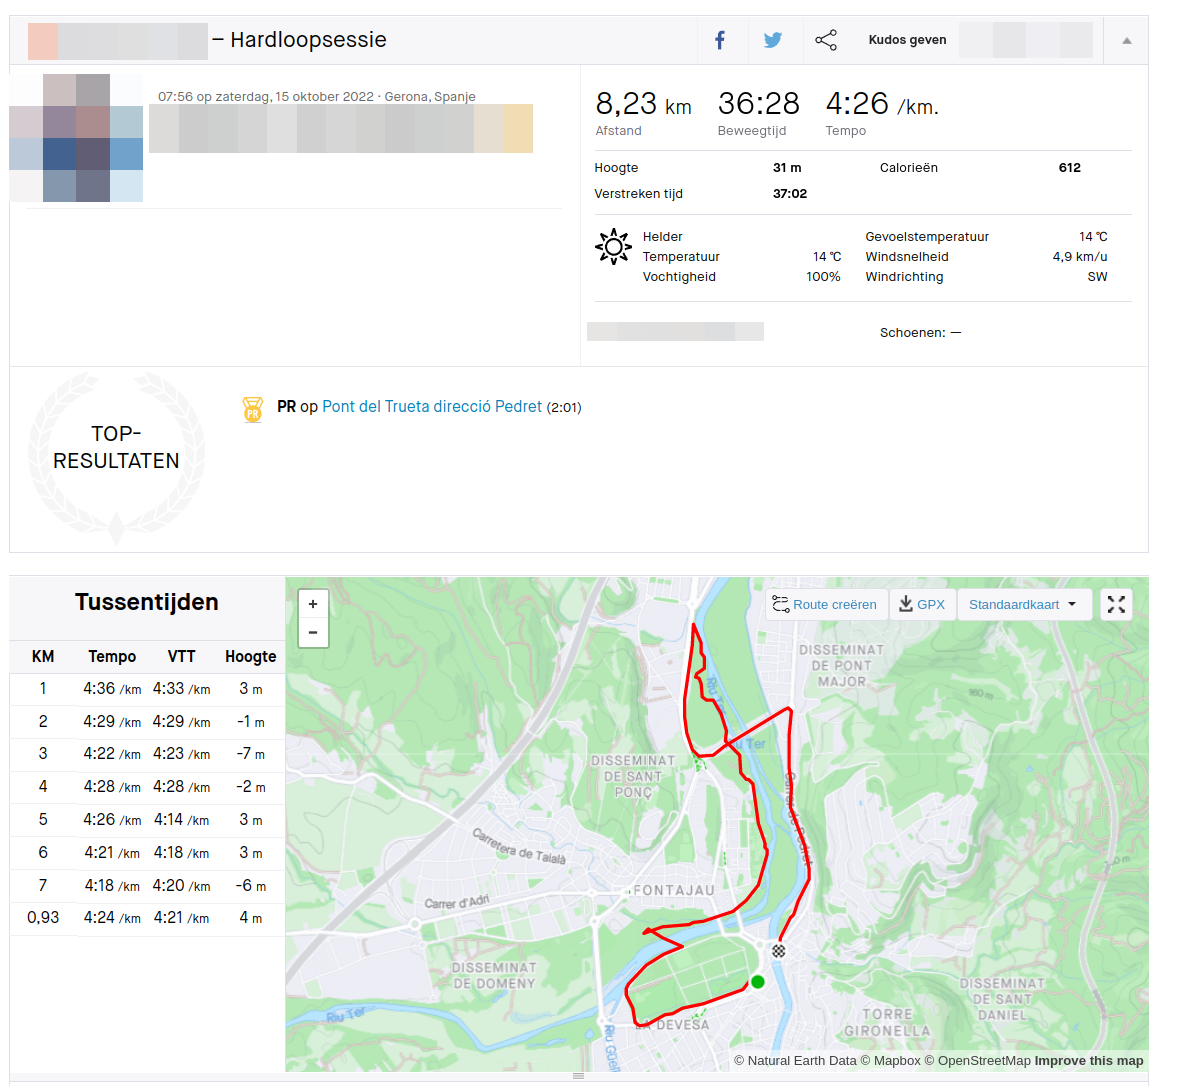
\includegraphics[width=0.5\linewidth]{fig/VoorbeeldActiviteiten/VoorbeeldActiviteit_Cropped.png}
    \caption{Voorbeeldactiviteit Strava}\label{fig:activityExample}
\end{figure}

Deze platformen implementeren elk manieren om de privacy van de users te
verbeteren. De meest eenvoudige te bedenken is misschien wel de mogelijkheid om
activiteiten te verbergen voor een selectie van personen (bv.\ iedereen die
geen volger is). Zo kunnen enkel de mensen die de gebruiker expliciet toelaat
activiteiten bekijken. Een complexer alternatief is het gebruik van \acp{EPZ}.
Hierbij wordt de weergegeven route voor de persoon die meekijkt gedeeltelijk
verborgen. Er wordt als het ware een deel van de route afgekapt. De echte
begin- en eindpunten zullen binnenin het afgekapte deel liggen. Er zullen
nieuwe punten worden gegenereerd worden, op de rand van de cirkel, die voor de
externe waarnemer het begin en einde zullen voorstellen. Het begin- en
eind-deel van de route wordt dus onzichtbaar voor de andere gebruikers. Door de
aanwezigheid van al deze pogingen tot privacyverbeteringen valt op dat de
ontwikkelaars van de platformen erg bewust zijn van de mogelijke gevaren.
Echter is er een afweging te maken bij de implementatie tussen de bruikbaarheid
van het platform, en de privacy van de eindgebruiker. Hoe meer data wordt
vrijgegeven, hoe groter de kans om mogelijk gevoelige info wordt meegegeven.
Aan de andere kant, bij het weglaten van informatie gaat de
gebruiksvriendelijkheid en de aanwezigheid van nuttige data van het platform
serieus achteruit.

\section{Doelstelling}
In dit onderzoek bekijken we of er een mogelijkheid bestaat om private locaties
(verborgen start- en eindlocaties) van een activiteiten te achterhalen, ondanks
het gebruik van de \ac{EPZ}~\ref{EPZ} als privacy beveiligingsmechanisme. In
het verleden werden enkele manieren beschreven om a.d.h.v.\ andere metadata
zoals hoogtedata en afstanden de \ac{EPZ} te omzeilen
(\textit{\cite{Dhondt_Pochat_Voulimeneas_Joosen_Volckaert_2022},\cite{Verdonck_2022}}).
Gedurende deze thesis wordt meer in detail gegaan op het gebruik van
snelheidsdata. Als basis voor deze aanval wordt de inferentie aanval op de EPZ
van~\citeauthor{Dhondt_Pochat_Voulimeneas_Joosen_Volckaert_2022} genomen. Er
wordt dan onderzocht of deze aanval nog steeds mogelijk is bij het weglaten van
bepaalde gegevens, en dus door het gebruik van andere gegevens. De focus ligt
in deze studie voornamelijk op snelheidsdata.

Om deze doelstelling te bekomen is eerst een berekeningsmechanisme nodig voor
de afstanden die nodig zijn om de inferentie-aanval te kunnen uitvoeren. Daarna
moet een analyse uitgevoerd worden tussen de berekende afstanden, en de waarden
afgeleid volgens de berekeningen
van~\citeauthor{Dhondt_Pochat_Voulimeneas_Joosen_Volckaert_2022}. Zo kan de
effectiviteit van de aanval a priori worden geschat. Er is een analyse van de
beschikbare data, en een bespreking en reflectie over de resultaten van de
aanval.
%%%%%%%%%%%%%%%%%%%%%%%%%%%%%%%%%%%%%%%%%%%%%%%%%%%%%%%%%%%%%%%%%%% 
%                                                                 %
%                            CHAPTER                              %
%                                                                 %
%%%%%%%%%%%%%%%%%%%%%%%%%%%%%%%%%%%%%%%%%%%%%%%%%%%%%%%%%%%%%%%%%%% 

\chapter{Achtergrond}

\section{Fitnesstrackers}
De focus van deze scriptie ligt op mogelijke tekortkomingen/vulnerabilities
betreffende privacybeleid in fitnesstrackers. Maar vooraleer we een aanval op
basis van deze kwetsbaarheden kunnen opzetten, is het noodzakelijk om een vat
te krijgen op welke manier een fitnesstracker info verzamelt en weergeeft, en
meer precies, hoe de mechanismen die de privacy voorzien voor de gebruikers in
detail werken.

De data waarmee de aanval wordt opgezet en waarmee wordt geëxperimenteerd, is
afkomstig van de populaire fitnesstracker
\textit{Strava\footnote{\url{https://www.strava.com/}}}. Dit is een sociaal
netwerk waarbij alle soorten sporters hun activiteiten kunnen delen. Dit gaat
over lopen, wandelen, fietsen, zwemmen, \ldots, maar ook sporten als fitnessen,
voetballen, \ldots De verzamelde data wordt volgens het perspectief van een
mogelijke aanval gefilterd, niet alle data blijkt nuttig te zijn. Enkel data
die gevoelige informatie met betrekking tot de woonplaats zou kunnen vrijgeven
wordt behouden. Dit zal er dus op neerkomen dat enkel activiteiten die
relevante \ac{gps}-informatie bevatten in beschouwing worden genomen. Dit gaat
dan meer specifiek over \textit{runs, hikes, walks, and rides}.

\subsection{Activiteiten}\label{data}
Een Strava-activiteit bevat erg veel informatie. Echter is niet alles even
bruikbaar. Een correcte abstractie van de onnodige data is dus nodig.
Figuur~\ref{fig:activityData} geeft een voorbeeld van een gedetailleerde
activiteit weer. Een gebruiker is in staat om de activiteit een titel te geven,
en er een korte beschrijving aan toe te voegen. Ook een foto kan optioneel
toegevoegd worden. De exacte datum en tijd van de start van de activiteit wordt
hierbij ook weergegeven.

Rechts daarvan zijn de algemene basisstatistieken te zien. Deze zijn de totale
afgelegde afstand, de totale bewegingstijd, de gemiddelde snelheid of het
gemiddelde tempo, het totale hoogteverschil, de totale verstreken tijden, en
het aantal calorieën verbrand. Als extra kunnen hier enkele statistieken
m.b.t.\ het gebruikte materiaal, zoals type fiets, loopschoenen, hartslagmeter,
enzovoort worden weergegeven. Een belangrijk onderscheid in deze context is het
verschil tussen de beweegtijd en de verstreken tijd. Deze twee lijken in
definitie gelijk, maar dit zijn ze niet. Strava, en fitnessplatformen in het
algemeen werken met twee verschillende soorten tijdsberekeningen voor het
bekomen van een accuratere gemiddelde snelheid of tempo. De verstreken tijd is
simpelweg het tijdsinterval tussen het vertrek van de activiteit en de
aankomsttijd ervan. De bewegingstijd is de tijd waarbij de gebruiker zich
effectief bewoog. Met andere woorden worden de tijden waarbij de gebruiker
stilstond uit de verstreken tijd gefilterd. Dit kan gaan over bijvoorbeeld een
pauze, of het wachten voor een verkeerslicht.

Er is een verschil bij fietsactiviteiten en wandelactiviteiten in hun weergave.
In het geval van een fietsactiviteit wordt \textit{snelheid} weergegeven, en in
het geval van een wandel- of loopactiviteit wordt \textit{tempo} weergegeven,
zoals te zien is op Figuur~\ref{fig:speedvspace}. Deze worden beide berekend
aan de hand van de bewegingstijd. Een kanttekening hierbij is dat dit enkel
geldt voor activiteiten die niet gelabeld zijn als \textit{race}, in dat geval
wordt de snelheid berekend in functie van de totaal verstreken
tijd~\cite{MovingTi80:online}. Het verschil tussen deze twee is dat de snelheid
wordt berekend volgens de formule $ \quad v = \frac{d}{t}$. De eenheid van
snelheid is dan ook $\frac{m}{s}$ of, in het geval van fitnesstrackers,
$\frac{km}{h}$. Het tempo wordt berekend volgens de formule $ \quad
    tempo(\frac{\min}{km}) = \frac{t(\min)}{d(km)}$. De eenheid van tempo is
$\frac{\min}{km}$. Om deze berekeningen wat te standaardiseren, werd gedurende
deze thesis gekozen om altijd de omrekening te maken naar tempo
$\frac{\min}{km}$, om zo over de volledige lijn met dezelfde standaard te
werken.
\begin{figure}[h]
    \centering
    \begin{subfigure}[b]{.5\textwidth}
        \centering
        \caption{Voorbeeldroute zonder map snapping}
        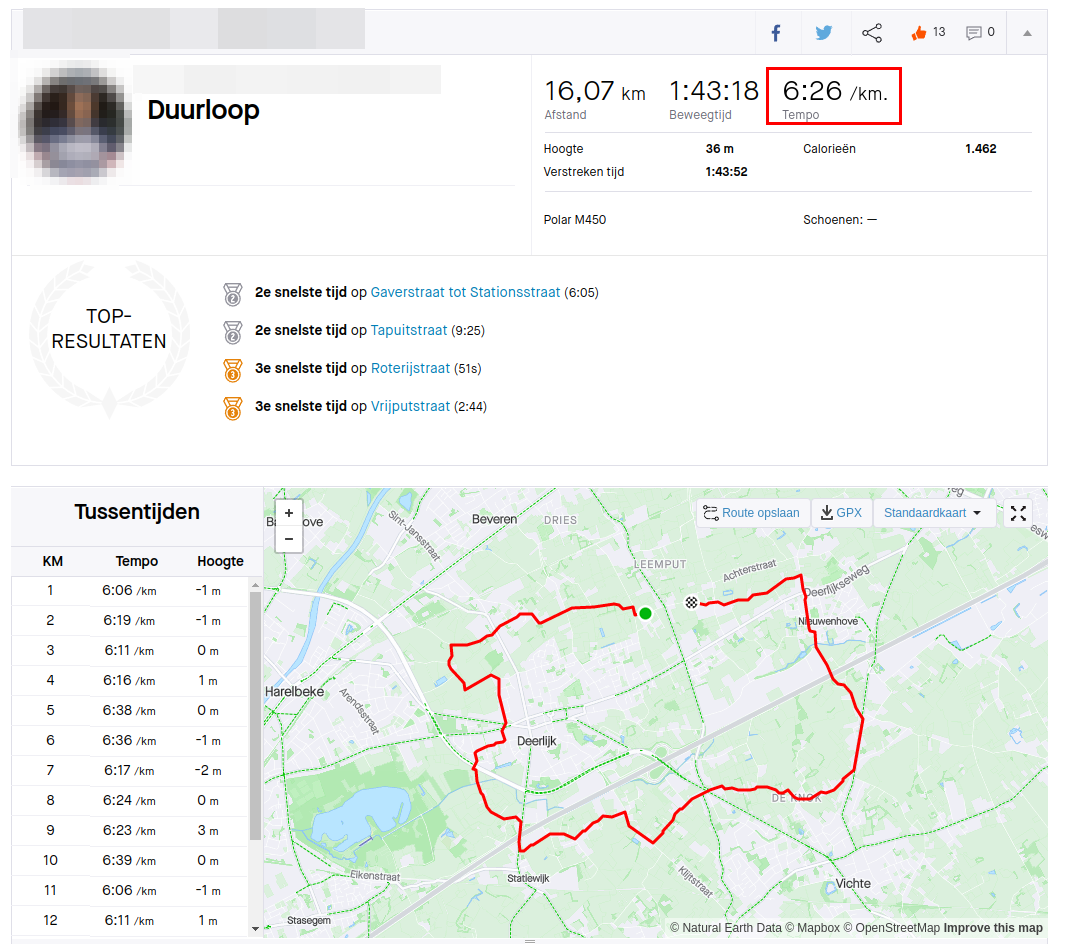
\includegraphics[width=\textwidth]{fig/SpeedVSPace/Pace.png}
    \end{subfigure}\hfill
    \begin{subfigure}[b]{.5\textwidth}
        \centering
        \caption{Fietsrit gebruikt snelheid}
        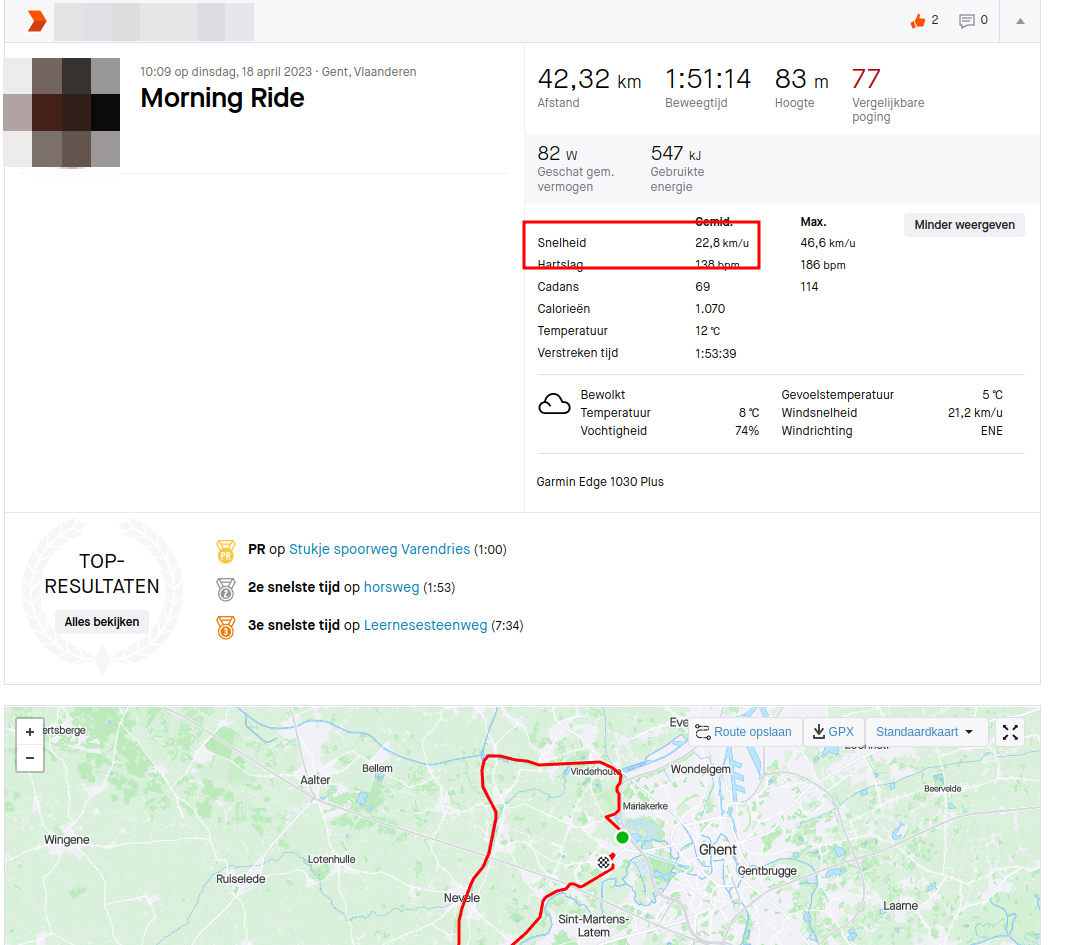
\includegraphics[width=\textwidth]{fig/SpeedVSPace/Speed.png}
    \end{subfigure}
    \caption{Verschil snelheid en tempo}\label{fig:speedvspace}
\end{figure}

Onder de basisstatistieken zijn de \textit{Strava-segmenten} te zien. Een
Strava-segment is een specifiek deel van een bepaalde route dat door gebruikers
van de sport-app kan worden gemarkeerd, gedeeld en vergeleken met andere
gebruikers. Het segment is een bepaalde afstand en route, bijvoorbeeld een klim
of afdaling, die vaak wordt beschouwd als een uitdagende of iconische sectie
van een bepaalde fiets- of hardlooproute. Gebruikers van Strava kunnen een
segment maken door de begin- en eindpunten op een kaart aan te geven en een
naam en beschrijving toe te voegen. Zodra het segment is gemaakt, kunnen andere
gebruikers het segment vinden en deelnemen aan een leaderboard, waarop de
snelste tijden worden bijgehouden en vergeleken met andere gebruikers.
Segmenten worden vaak gebruikt om prestaties te meten en te vergelijken.

Centraal op de figuur is ook de kaart duidelijk zichtbaar. Daarbij horen ook de
tussentijden en de grafiek van snelheid. Optioneel kan hierbij ook nog een
visualisatie van de afgelegde hoogte en de hartslag worden weergegeven, indien
de gebruiker hiervoor met de juiste meetinstrumenten zijn sportactiviteit
opneemt. De tussentijden en de grafiek van snelheid zijn qua inhoud
gelijkaardig, met als verschil dat de waarden op de grafiek erg precies kunnen
worden bestudeerd. Op de grafiek is voor elk afstandspunt de ogenblikkelijke
snelheid zichtbaar. Bij de tussentijden wordt de gemiddelde snelheid over een
kilometer weergegeven. De kaart die de route weergeeft is zeker ook belangrijk
om even te bestuderen. Deze bevat namelijk alle \ac{gps}-geregistreerde punten,
en verbindt deze ook om zo één aaneensluitende route te vormen. Wanneer deze
echter in detail bestudeerd wordt, samen met de legende die aanwezig is, is te
zien dat de route uit twee delen bestaat, een zichtbaar deel en een onzichtbaar
deel. Een andere gebruiker zal enkel zicht hebben op de het zichtbare deel, het
onzichtbare deel zal dus voor een andere gebruiker niet zichtbaar zijn. Anders
geformuleerd, de activiteit zal voor deze persoon dus als het ware afgekapt
zijn, en zal in zijn zichtbare versie op een andere plek starten en eindigen.
In de volgende Secties~\ref{sec:Algemene Privacy} \&~\ref{sec:EPZ} wordt meer in
detail ingegaan op de werking van deze methodiek.

Een laatste kanttekening die hierbij gemaakt moet worden, is dat voor een
gebruiker verschillende eenheden mogelijk zijn om uit te kiezen. Er is keuze
mogelijk tussen de mijl en pond, en kilometer en kilogram. Gebruikers kiezen in
welke eenheid ze de applicatie wensen te gebruiken. Voor de gebruiker in
kwestie zal dus de volledige applicatie worden weergegeven in de gekozen
eenheden.
\begin{figure}
    \centering
    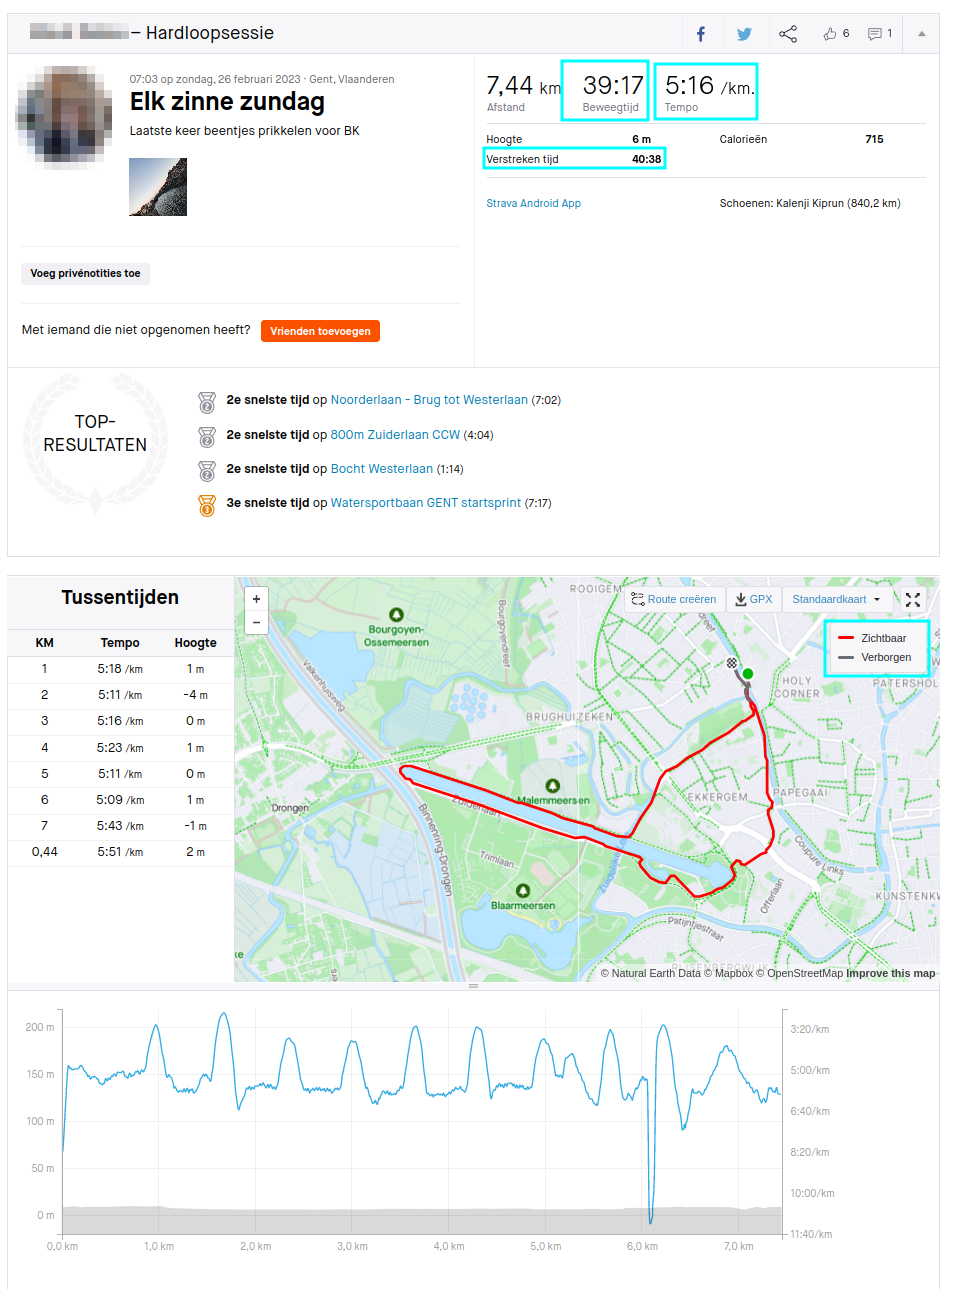
\includegraphics[width=0.8\textwidth]{fig/VoorbeeldActiviteiten/VoorbeeldActiviteit_Personal.png}
    \caption{Data van een activiteit}\label{fig:activityData}
\end{figure}

\subsection{Berekening Afstanden}\label{sec:afstandsberekeningen_strava}
Fitnesstrackers krijgen vanuit de buitenwereld ruwe data binnen. Deze data moet
dus verwerkt worden vooraleer ze bruikbaar is voor de gebruiker. Er werd al
kort ingegaan in Sectie~\ref{data} op de berekening die Strava gebruikt voor de
snelheid. Echter is het ook interessant om de berekening van Strava eens onder
de loep te nemen voor de afgelegde afstand. Strava maakt gebruik van twee
verschillende methodieken voor het berekenen van deze afstand. De eerste is de
\textit{GPS-calculated Distance}. Dit bestaat eruit om de afstand tussen
opeenvolgende \ac{gps}-punten te berekenen, en deze op te tellen. Precisie is
hier afhankelijk van de precisie van de \ac{gps}-punten, aangezien de afstand
wordt berekend door de punten met rechte lijnen te verbinden. Dit kan gebeuren
in real time, via de gsm, smartwatch of ander toestel die gebruikt wordt om de
activiteit op te nemen. Er zal dan ook mogelijkheid zijn om real time info te
zien. Op elk punt zal de afstand vanaf het startpunt gekend zijn, en het is
deze afstand die gedeeld zal worden op het platform. Het grote nadeel hierbij
is het real-time aspect. Fouten kunnen moeilijker on the fly worden
gecorrigeerd. Een tweede aanpak is om \ac{gps}-data pas bij het uploaden te
verwerken. De \ac{gps}-data wordt dan geanalyseerd, en de nodige berekeningen
worden uitgevoerd.

Het alternatief voor de GPS-calculated distance is de \textit{Ground Speed
    Distance} methodiek. Deze afstand kan enkel worden bepaald in het geval van een
fietsactiviteit met behulp van een capabele fietscomputer die omwentelingen van
de wielen kan meten. De fietscomputer berekent dan de afstand door het aantal
omwentelingen te vermenigvuldigen met de omtrek van het
fietswiel~\cite{HowDista47:online}.

De bovenstaande afstandsberekeningen zijn de twee technieken die de officiële
supportdocumentatie van Strava beschrijft~\cite{HowDista47:online}. Echter
blijkt wanneer we de afstand op deze manier manueel berekenen, afwijkende
resultaten bekomen worden. Dit is zeer waarschijnlijk te wijten aan de
preprocessing van de data die gebeurt bij het uploaden van een activiteit.
Alhoewel dit niet expliciet gedocumenteerd staat doen de resultaten dit wel
sterk vermoeden. De hypothese is dat tijdens het uploaden, de afstand
herberekend wordt. De \ac{gps}-punten zullen worden geanalyseerd, en er zullen
technieken worden gebruikt om de resultaten hiervan te verbeteren. De twee
meest waarschijnlijke technieken zijn \textit{Map Snapping} en
\textit{Smoothing}.

Map Snapping of Snap to Roads is een techniek waarbij \ac{gps}-punten worden
verschoven naar de dichtstbijzijnde weg. Per \ac{gps}-punt wordt dan gezocht
naar de dichtste node op de desbetreffende \textit{roadgraph}\footnote{De
    roadgraph is afhankelijk van welke implementatie gebruikt wordt voor het
    snappen. Het is een wegennetwerk, omgezet in een graaf, bestaande uit edges en
    nodes. Elke weg of pad, bevat één of meerdere nodes, zodat een skeletstructuur
    ontstaat, die een abstractie van het wegennetwerk
    voorstelt~\cite{seiler2022haul}}, op Figuur~\ref{fig:MapSnapping} is de werking
ervan te zien~\cite{Snapping96:online}.
\begin{figure}[h]
    \centering
    \begin{subfigure}[b]{.5\textwidth}
        \centering
        \caption{Voorbeeldroute zonder map snapping}
        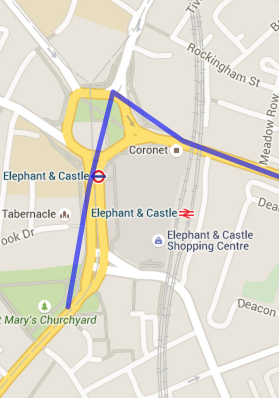
\includegraphics[width=0.5\textwidth]{fig/Map Snapping/before.png}\label{fig:before_MapSnapping}
    \end{subfigure}\hfill
    \begin{subfigure}[b]{.5\textwidth}
        \centering
        \caption{Voorbeeldroute met map snapping}
        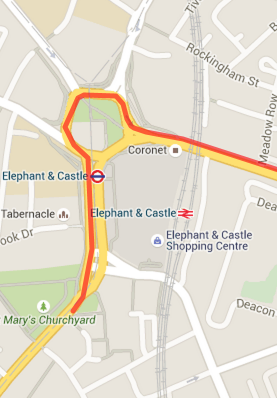
\includegraphics[width=0.5\textwidth]{fig/Map Snapping/after.png}\label{fig:after_MapSnapping}
    \end{subfigure}
    \caption{Voorbeeld van de werking van \textit{Map Snapping}}\label{fig:MapSnapping}
\end{figure}

Daarnaast bestaat de kans dat er gebruik gemaakt wordt van smoothing. Smoothing
is een proces dat ruwe \ac{gps}-punten (of datapunten in het algemeen) op een
traject probeert te optimaliseren opdat ze een vloeiend `curve' vormen. Dit
wordt bekomen door ruis, schommelingen en onnauwkeurigheden te filteren uit het
traject. Hiervoor bestaan verschillende implementaties. Aangezien Strava geen
openbare informatie verstrekt over het gebruik van gps-smoothing, is het niet
bekend of ze deze techniek effectief toepassen. Het is dus gissen naar, indien
ze deze zouden gebruiken, welke implementatie dan wel gebruikt wordt. De
makkelijkste en meest modulaire methode om aan smoothing te doen, is
\textit{Smoothing met Moving Average}. Deze methode bestaat eruit om van een
aantal punten in een bepaalde range (ook `window' genoemd) het gemiddelde te
nemen, en vervolgens op te schuiven. Het gemiddelde wordt berekend met volgende
formule: $\overline{y_x} = \frac{y_x + y_{x+1} + \ldots + y_{x+n}}{x+n}$, voor
punt x, met n als window-grootte~\cite{Smoothin16:online,
    SmoothingandInterpolatingNoisyGPSDatawithSmoothingSplines, Smoothin86:online}.
Zo kan voor elk punt een evenwichtige waarde op de nieuwe grafiek bekomen
worden, en krijgt de grafiek een meer vloeiende vorm. Merk wel op dat de
precisie van de route afneemt op deze manier. Bij het smoothen van een traject
wordt het aantal gebruikte punten namelijk verminderd volgens de grootte van de
window. Afhankelijk van de grootte, worden meer (resp.\ minder) punten
samengenomen, en zo minder/meer punten weergegeven op de grafiek. Een voorbeeld
is terug te vinden op Figuur~\ref{fig:SmoothingExample}, waarbij de blauwe
curve de ruwe data voorstelt, dus voorafgaand op het `smoothen', en de rode de
`gesmoothe' curve.
\begin{figure}[h]
    \centering
    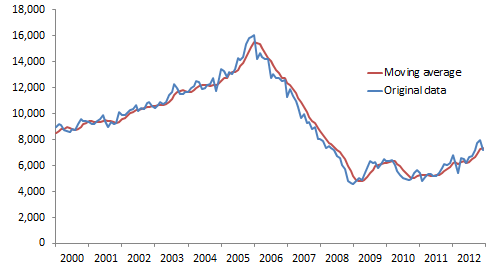
\includegraphics[width=0.6\linewidth]{fig/SmoothingExample.png}
    \caption{Voorbeeld Data smoothing with moving average}\label{fig:SmoothingExample}
\end{figure}
% - https://support.strava.com/hc/en-us/articles/216917707-Bad-GPS-Data

\subsection{Algemeen Privacybeleid}\label{sec:Algemene Privacy}
Het is zeker niet altijd wenselijk om alle data die vervat zit in zo'n
activiteit met alle andere gebruikers op het platform te delen. De
ontwikkelaars kiezen er dan ook voor om gebruikers de mogelijkheid te geven om
hun privacy te bewaren. In deze sectie wordt de focus gelegd op de mechanismen
gebruikt door \textit{Strava}. Als opmerking valt te melden dat in heel wat
andere sport-applicaties vergelijkbare, zo niet dezelfde methodieken worden
gebruikt. Een eerste algemeen mechanisme bestaat eruit om de gebruiker de keuze
te geven om alle activiteiten en alle gegevens over het profiel heen te laten
voldoen aan bepaalde privacy regels. Deze regels kunnen ook per activiteit
worden ingesteld. Onder de keuzes staan meestal drie opties, \textit{zichtbaar
    voor iedereen}, \textit{zichtbaar voor volgers} en \textit{zichtbaar voor
    niemand}. Er kan ook zelf een keuze gemaakt worden om specifieke elementen van
een activiteit niet te delen met de buitenwereld, zoals bijvoorbeeld de
zichtbaarheid van de route op de kaart~\cite{Activity24:online}.

\section{Endpoint Privacy Zones}\label{sec:EPZ}
Een tweede belangrijke maatregel is het gebruik van de de \acp{EPZ}. Een
\ac{EPZ} is een cirkelvormige zone met een bepaalde straal rond een
\ac{gps}-punt. Het punt in kwestie zal dus de betreffende \textit{gevoelige
    locatie} zijn. De straal van deze cirkel\footnote{Op Strava heeft de \ac{EPZ}
    de vorm van een cirkel, maar op andere platformen kunnen andere vormen de norm
    zijn, bv.\ polygonen.} kan worden gekozen door de gebruiker, en in het geval
van Strava hebben gebruikers keuze uit waarden van 0 tot 1600m, in stappen van
200m. Wanneer een gebruiker binnen deze zone zijn activiteit beëindigt of
begint, dan zal dat deel van de route binnen de \ac{EPZ} niet zichtbaar zijn
voor anderen. Vanuit het perspectief van een andere gebruiker zal de activiteit
dus starten en/of eindigen op de rand van deze cirkel (die natuurlijk niet
zichtbaar is). Merk op dat een sporter ook andere gevoelige locaties kan
verbergen op de kaart. Bijvoorbeeld een frequent bezocht café, of een huis van
een partner waar regelmatig een tussenstop plaatsvindt. Een tweede opmerking is
dat wanneer een gebruiker de \ac{EPZ} doorkruist, maar er niet in stopt, dat
deel van de route onaangepast blijft. Op Figuur~\ref{fig:EPZ_Voorbeeld} zijn de
verschillende perspectieven te zien, hoe het er als uploader uitziet, en hoe
het eruit ziet voor een andere gebruiker. Het traject dat de buitenstaander te
zien krijgt, bestaat uit alle punten die zich buiten de \ac{EPZ} bevinden. Merk
ook op dat de eigenaar van de activiteit zicht heeft op de invloed van de
\ac{EPZ}, dus wat zal verborgen worden erdoor, en wat zichtbaar blijft. Dit
onderscheid wordt gemaakt door het verschil in kleur, oranje voor de publiek
zichtbare punten en grijs voor de onzichtbare.
\begin{figure}[h]
    \centering
    \begin{subfigure}[b]{.49\textwidth}
        \centering
        \caption{Perspectief eigenaar}
        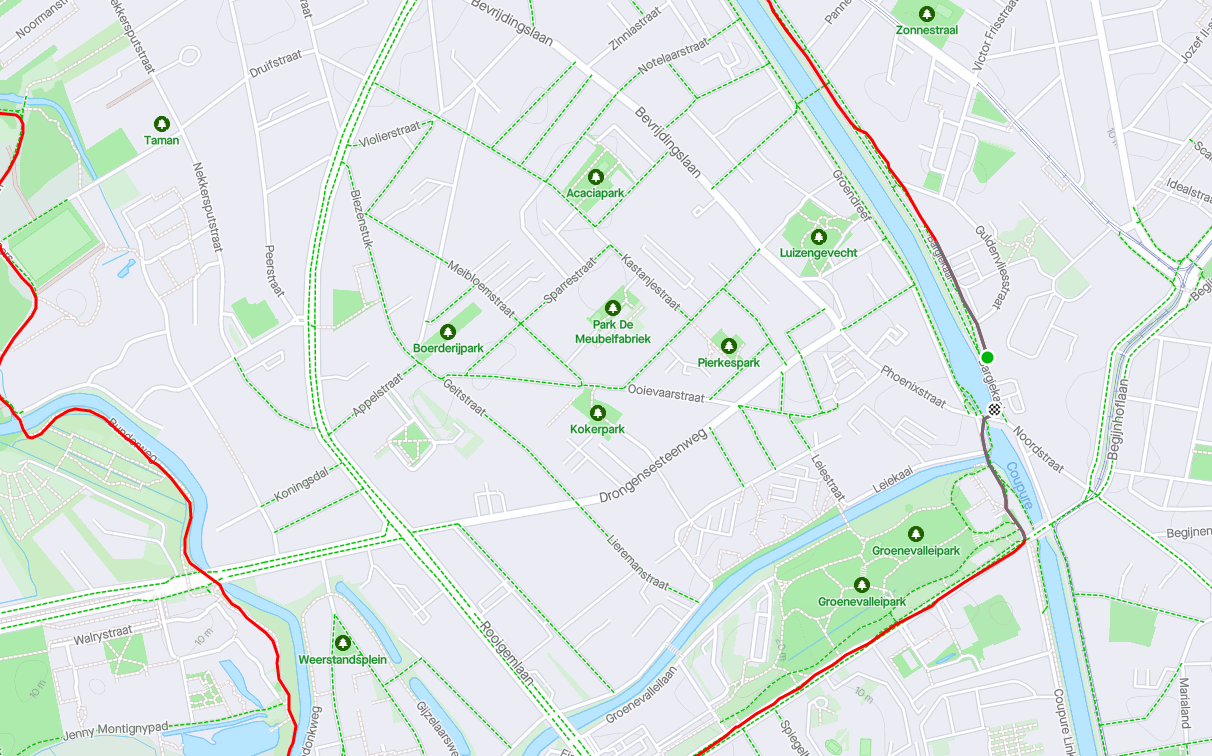
\includegraphics[width=1\textwidth]{fig/EPZ-mechanisme/Example_EPZ_InternalView.png}\label{fig:EPZ_internal}
    \end{subfigure}\hfill
    \begin{subfigure}[b]{.49\textwidth}
        \centering
        \caption{Perspectief externe gebruiker}
        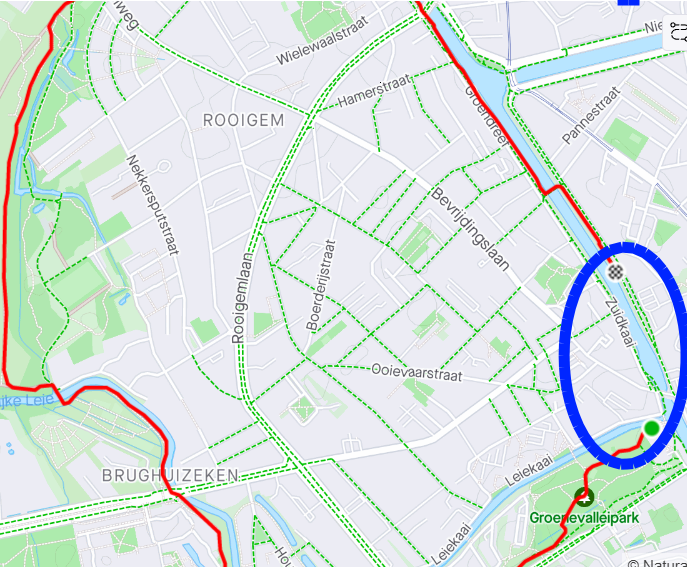
\includegraphics[width=1\textwidth]{fig/EPZ-mechanisme/Example_EPZ_ExternalView.png}\label{fig:EPZ_external}
    \end{subfigure}
    \caption{Voorbeeld van de werking van een \ac{EPZ}}\label{fig:EPZ_Voorbeeld}
\end{figure}

De methodiek die fitnesstrackers toepassen bij het opzetten van een \ac{EPZ}
werkt als volgt, de gevoelige locatie wordt genomen als beginlocatie. Hieruit
zal a.d.h.v.\ de op voorhand vastgelegde \ac{EPZ}-straal een cirkel worden
opgesteld. Het centrum van deze cirkel zal hierna een translatie ondervinden in
een willekeurige richting. Dit kan een verschuiving zijn met een afstand die
maximaal 70\% van de straal van de \ac{EPZ} bedraagt. Dit mechanisme is te zien
op Figuur~\ref{fig:translation}. Het transleren van deze cirkel wordt ook
\textit{spatial cloaking} genoemd.
\begin{figure}[h]
    \centering
    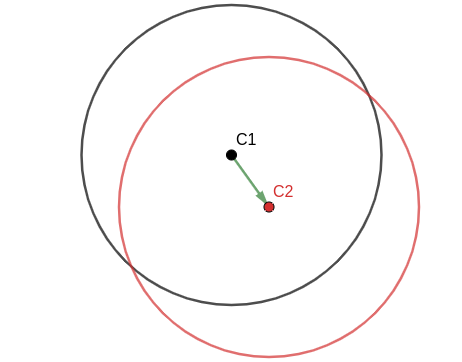
\includegraphics[width=0.4\linewidth]{fig/EPZ-mechanisme/Translation_Center.png}
    \caption{Voorbeeld translatie EPZ}\label{fig:translation}
\end{figure}

Daarna worden alle punten vertrekkende vanaf de gevoelige locatie tot aan de
rand van de \ac{EPZ}, en vanaf de rand van de \ac{EPZ} tot aan de gevoelige
locatie verwijderd van het zichtbare traject. Merk op dat punten die de
\ac{EPZ} doorkruisen, maar niet vertrekken of aankomen bij de gevoelige locatie
niet worden gefilterd. Een voorbeeld van deze filtering is te zien op
Figuur~\ref{fig:drop points}.
\begin{figure}[h]
    \centering
    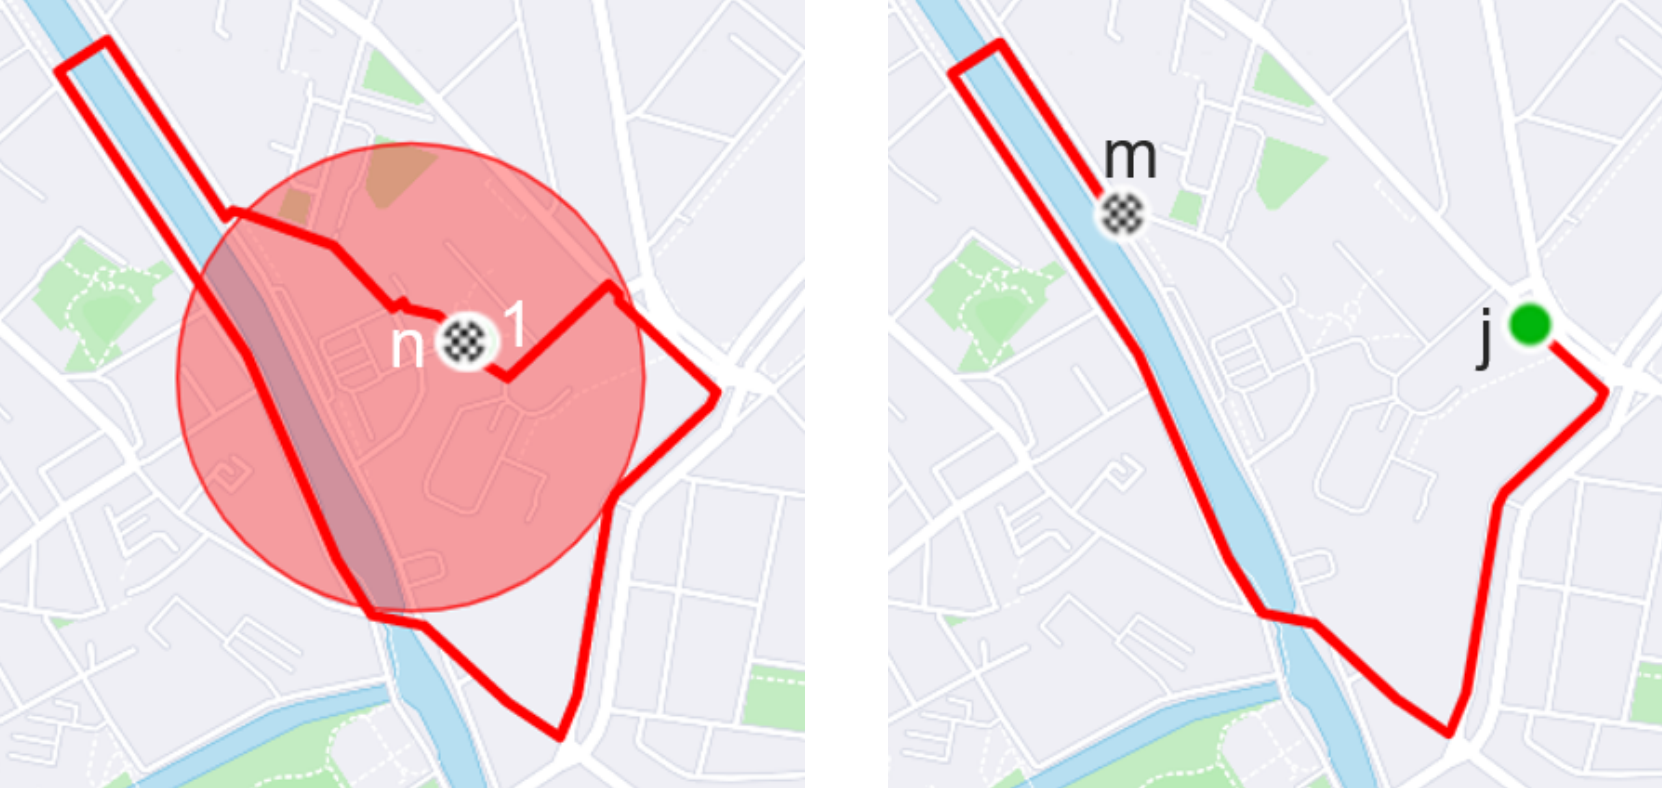
\includegraphics[width=0.7\linewidth]{fig/EPZ-mechanisme/DropEPZPoints.png}
    \caption{Voorbeeld filtering van punten binnen \ac{EPZ}}\label{fig:drop points}
\end{figure}

\section{Literatuur}
In het verleden is al wat onderzoek verricht in de richting van de
doeltreffendheid van \acp{EPZ} bij fitnesstrackers. Hassan et al.\ beschreef in
2018 een implementatie van EPZ waarbij het centrum van de zone de gevoelige
locatie is. M.a.w.\ het identificeren van deze zone is dus voldoende om de
gevoelige locatie te achterhalen~\cite{sec18has3:online}. In tegenstelling tot
deze thesis, wordt ervan uitgegaan dat het centrum geen translatie ondervindt,
en er dus geen spatial cloaking wordt toegepast. In deze paper wordt gefocust
op de reconstructie van de cirkel op basis van 3 punten op de rand, wat te zien
is op Figuur~\ref{fig:Hassan_EPZ}. Deze 3 randpunten worden dus bekomen door
begin/eindpunten te nemen van activiteiten, volgens het perspectief van
gebruiker die geen eigenaar is. Deze begin/eindpunten zullen zich altijd op de
rand van de cirkel begeven. Door het toepassen bekwam Hassan et al.\ een succes
rate tot 95.1 Spatial cloaking werd er aangehaald als mogelijke verdediging
tegen dit soort aanvallen.
\begin{figure}[h]
    \centering
    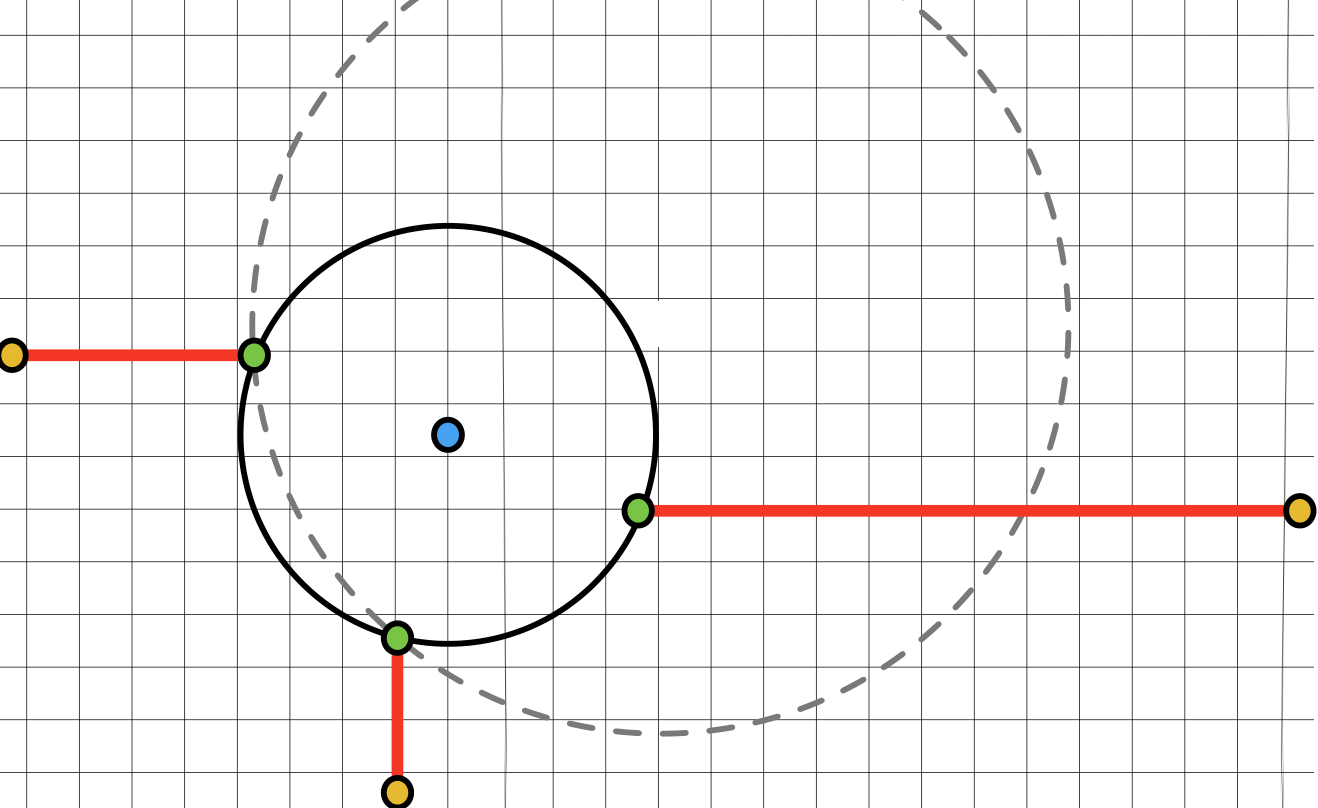
\includegraphics[width=0.6\textwidth]{fig/EPZ-mechanisme/Hassan.png}
    \caption{Mechanisme \ac{EPZ} beschreven door Hassan et al.}\label{fig:Hassan_EPZ}
\end{figure}

Een onderzoek door~\citeauthor{10.1145/3491102.3502136} in 2022 toonde ook aan
dat heel wat mensen in staat zijn om de gevoelige locatie te achterhalen op
basis van hun intuïtie~\cite{10.1145/3491102.3502136}. Dit gebeurde op basis
van enquêtes die werden afgenomen bij gebruikers van het platform. Deelnemers
aan de enquête moesten op basis van activiteiten opgenomen door een
fitnesstracker, die verhuld waren gebruik makend van spatial cloaking, de
startlocatie van een gebruiker proberen te achterhalen. Uit het onderzoek bleek
dat 68\% van de ondervraagden bij een \ac{EPZ}-radius van 200m de beschermde
locatie tot op 50m nauwkeurig konden voorspellen. Hoe meer activiteiten ter
beschikking zijn, hoe effectiever de deelnemers de locatie konden schatten.
Deze resultaten op zich zijn alarmerend, en tonen aan dat \acp{EPZ} verre van
perfect zijn, en ook te omzeilen zijn door een persoon die geen technische
achtergrond heeft.

Dhondt et al.\ voerde tevens ook een studie in 2022 naar de mogelijke lekken
aanwezig in het principe van
\acp{EPZ}~\cite{Dhondt}. Er wordt in
deze paper een nadruk gelegd op de translatie van de \ac{EPZ}, en hoe deze de
privacy van een gebruiker verhoogt. Een inferentie aanval, wordt er beschreven
die gebruikmaakt van de totale afstand die terug te vinden bij de activiteit.
Het principe van deze inferentie aanval wordt uitvoerig beschreven in
Sectie~\ref{chap:inferentieaanval}. In het kort werkt de aanval als volgt: aan
de hand van de totale afgelegde afstand in combinatie met het wegennetwerk in
die omgeving, wordt een poging gedaan om alle mogelijke routes die de sporter
binnenin de \ac{EPZ} zou kunnen afgelegd hebben te reconstrueren. Dit gebeurt
voor elke activiteit. Wanneer dit gedaan wordt voor verschillende trajecten,
kan een locatie voorspeld worden die het meest waarschijnlijk wordt geacht om
de gevoelige locatie te zijn.

Deze aanpak toonde aan dat de beschreven countermeasure door Hassan et al.\
niet feilloos is, en dat deze kan worden omzeild met een successrate van 85\%.
Aangezien activiteiten nog steeds totale afstanden van een volledige route
vrijgeven, kan de afstand afgelegd binnenin de EPZ geïnfereerd worden. Deze
data ligt dan ook aan de grond van de inferentie aanval volgens Dhondt et al.

Het meest recente werk in dit domein is de thesis
van~\citeauthor{Verdonck_2022}~\cite{Verdonck_2022}. Deze thesis bouwt in grote
mate verder op de paper van
\citeauthor{Dhondt}, maar er wordt
alternatieve data gebruikt. Er wordt een onderzoek gedaan in hoeverre de
resultaten kunnen worden bekomen door het gebruik van hoogtedata om beschermde
locaties te achterhalen. Via de kennis van hoogtedata van het stratenplan kan
via de gekende hoogteverschillen een inferentie aanval opgezet worden, die nu
geen afstanden maar hoogteverschillen infereerd. Op deze manier
bekomt~\citeauthor{Verdonck_2022} een succes rate van 36\%. Dit lagere
succesratio is terug te brengen naar het feit dat hoogtedata een stuk minder
precies zijn. Ook is hoogtetoename in heel wat regios niet zo significant, wat
de succesrate niet ten goeie komt.
%%%%%%%%%%%%%%%%%%%%%%%%%%%%%%%%%%%%%%%%%%%%%%%%%%%%%%%%%%%%%%%%%%% 
%                                                                 %
%                            CHAPTER                              %
%                                                                 %
%%%%%%%%%%%%%%%%%%%%%%%%%%%%%%%%%%%%%%%%%%%%%%%%%%%%%%%%%%%%%%%%%%% 

\chapter{Setting aanval}\label{chap:inferentieaanval}
In dit hoofdstuk beschrijven we de setting alsook de werking van de aanval. De
aanval is sterk gebaseerd op de aanvallen van~\citeauthor{Dhondt}
en~\citeauthor{Verdonck_2022}~\cite{Verdonck_2022, Dhondt}. Deze aanvallen
worden inferentieaanvallen genoemd, vanwege het feit dat uit metadata
essentiële gegevens kunnen worden geïnfereerd. In het geval
van~\citeauthor{Dhondt} gaat dit over afgelegde afstand binnenin de \ac{EPZ}.
In het geval van~\citeauthor{Verdonck_2022} gaat dit dan weer over geïnduceerde
hoogteverschillen binnen de privacy zone. Allereerst zullen we kort de
mogelijkheden van een aanvaller in de huidige setting bespreken. Daarna wordt
de inferentieaanval van~\citeauthor{Dhondt}, die de basis vormt voor de aanval
in deze thesis, besproken volgens een opdeling in drie stappen.

\section{Definitie aanvaller}\label{sec:definitie-aanvaller}
Deze thesis voert een onderzoek naar de mogelijkheid om een \ac{EPZ} te
omzeilen. De studie wordt dus gevoerd vanuit het opzicht van een aanvaller.
Vooraleer we de werking van een aanval kunnen beschreven, is het belangrijk om
een zicht te hebben op het doel en de capaciteiten van een aanvaller.

Hier is een aanvaller een gebruiker van het platform die geen eigenaar is van
een activiteit. Hij heeft echter wel zicht op alle metadata die publiekelijk
gedeeld is. Dit is data zoals afgelegde afstand, snelheid, tempo, \ldots \
Aangezien de aanval gaat over het omzeilen van \acp{EPZ} worden enkel
activiteiten beschouwd die gecloaked zijn. De aanvaller heeft dus geen zicht op
de reële start- en/of eindlocatie. Zijn of haar doel is dan ook om ondanks de
aanwezigheid van cloaking deze gevoelige locatie te achterhalen.

Vanuit het oogpunt van de inferentieaanval beschreven door~\citeauthor{Dhondt}
heeft de aanvaller toegang tot alle data die publiek beschikbaar is. In deze
aanval wordt echter wel voornamelijk gebruik gemaakt van afstandsdata. De
aanvaller die we in deze thesis beschrijven, heeft echter geen toegang tot deze
afstandsdata. Hij heeft wel nog toegang tot de ruwe gps-data, maar ook de
snelheid, het tempo enzovoort. Het onderzoek bestaat er dus uit om te zien in
hoeverre een aanval nog mogelijk is wanneer de afstandsdata onbruikbaar zou
zijn. We onderzoeken dus een alternatieve aanpak om de inferentieaanval alsnog
succesvol te kunnen uitvoeren.

We beschrijven de aanvaller vanuit een theoretisch kader. We bestuderen onder
welke omstandigheden de aanval mogelijk is, en welke maatregelen effectief
blijken. Het globale scenario waar we van uitgaan is: `wat als fitnesstrackers
de afstandsgegevens op een bepaalde manier zouden verbergen of onbruikbaar
maken, door bijvoorbeeld afrondingen te maken, of onzekerheid toe te voegen'.
Is de aanval dan nog mogelijk, en zo ja, hoe effectief is deze dan nog, en wat
voor gevolgen heeft dit ten opzichte van eerder bespoken
beschermingsmaatregelen?

\subsection{Assumpties}\label{sec:assumpties}
Om de aanval te kunnen uitvoeren, moeten enkele assumpties worden gemaakt.
\citeauthor{Dhondt} maakten al enkele assumpties om de inferentieaanval
succesvol uit te voeren. Voor dit onderzoek is het dus logisch om dezelfde
veronderstellingen te maken. Zo kunnen we een nuttige vergelijking maken. De
eerste assumptie stelt dat de zichtbare begin -en eindpunten op de rand van de
\ac{EPZ} moeten liggen. Ten tweede moet de beschermde locatie op de roadgraph
liggen. Hij kan niet buiten het voor ons te mappen gebied liggen, bijvoorbeeld
in een bos waar geen pad in kaart is gebracht. Er wordt dieper ingegaan op de
roadgraph in Sectie~\ref{sec:roadgraph}. Als laatste, maar desalniettemin
belangrijk punt moet de gebruiker binnenin de \ac{EPZ} de kortste route
volgen~\cite{Dhondt}.

Dhondt et al.\ maakte nog een laatste assumptie betreffende start- en
eindpunten, meer bepaald dat deze die dezelfde locaties moeten voorstellen. Dit
is echter niet van toepassing op dit onderzoek. Het onderzoek focust zich op
activiteiten waar slechts één deel van het traject verborgen is. Dit wil dan
ook zeggen dat de gebruiker ofwel vertrekt op de gevoelige locatie, of er
eindigt, maar niet beide. Op Figuur~\ref{fig:totalDistanceAttack} zijn de 2
mogelijke scenarios van een total distance attack terug te vinden, namelijk
waarbij ofwel gestart als geëindigd wordt binnenin de zone. Dit wordt ook een
\textit{total distance attack} genoemd, omdat enkel de totale afstand en de
afstand buiten de \ac{EPZ} nodig is. Op deze figuur zijn de rode punten
gelabeld \textit{Start} en \textit{End} de zichtbare start- en eindpunten. Dit
scenario stelt dat één van de reële start- of eindpunten de gevoelige locatie
is, aangeduid met de zwarte markering. Een andere aanval is de \textit{inner
    distance attack}, hierbij zullen zowel de start als het einde van een
activiteit binnenin het te verbergen gebied liggen, dit is te zien op
Figuur~\ref{fig:innerDist}. De kennis van de afzonderlijke afstand die de
gebruiker aflegt van de effectieve startlocatie tot de rand van de \ac{EPZ} en
van de rand van de \ac{EPZ} tot de effectieve eindlocatie is dan ook een
vereiste. Op de Figuur zijn opnieuw de zichtbare randpunten aangeduid in het
rood. Echter zal het onzichtbare traject voor beide gevallen doorlopen en
eindigen op de gevoelige locatie, wat in dit geval de reële start- en
eindlocatie is. In Sectie~\ref{sec:berekeningen} wordt dieper ingegaan op de
reden waarom een \textit{inner distance attack} niet mogelijk is. In deze
thesis worden dus alle activiteiten waarvan enkel een verhulde start- of
eindlocatie behouden, de rest wordt gefilterd in deze context.
\begin{figure}[h]
    \centering
    \begin{subfigure}[b]{.5\textwidth}
        \centering
        \caption{Start binnenin de \ac{EPZ}}
        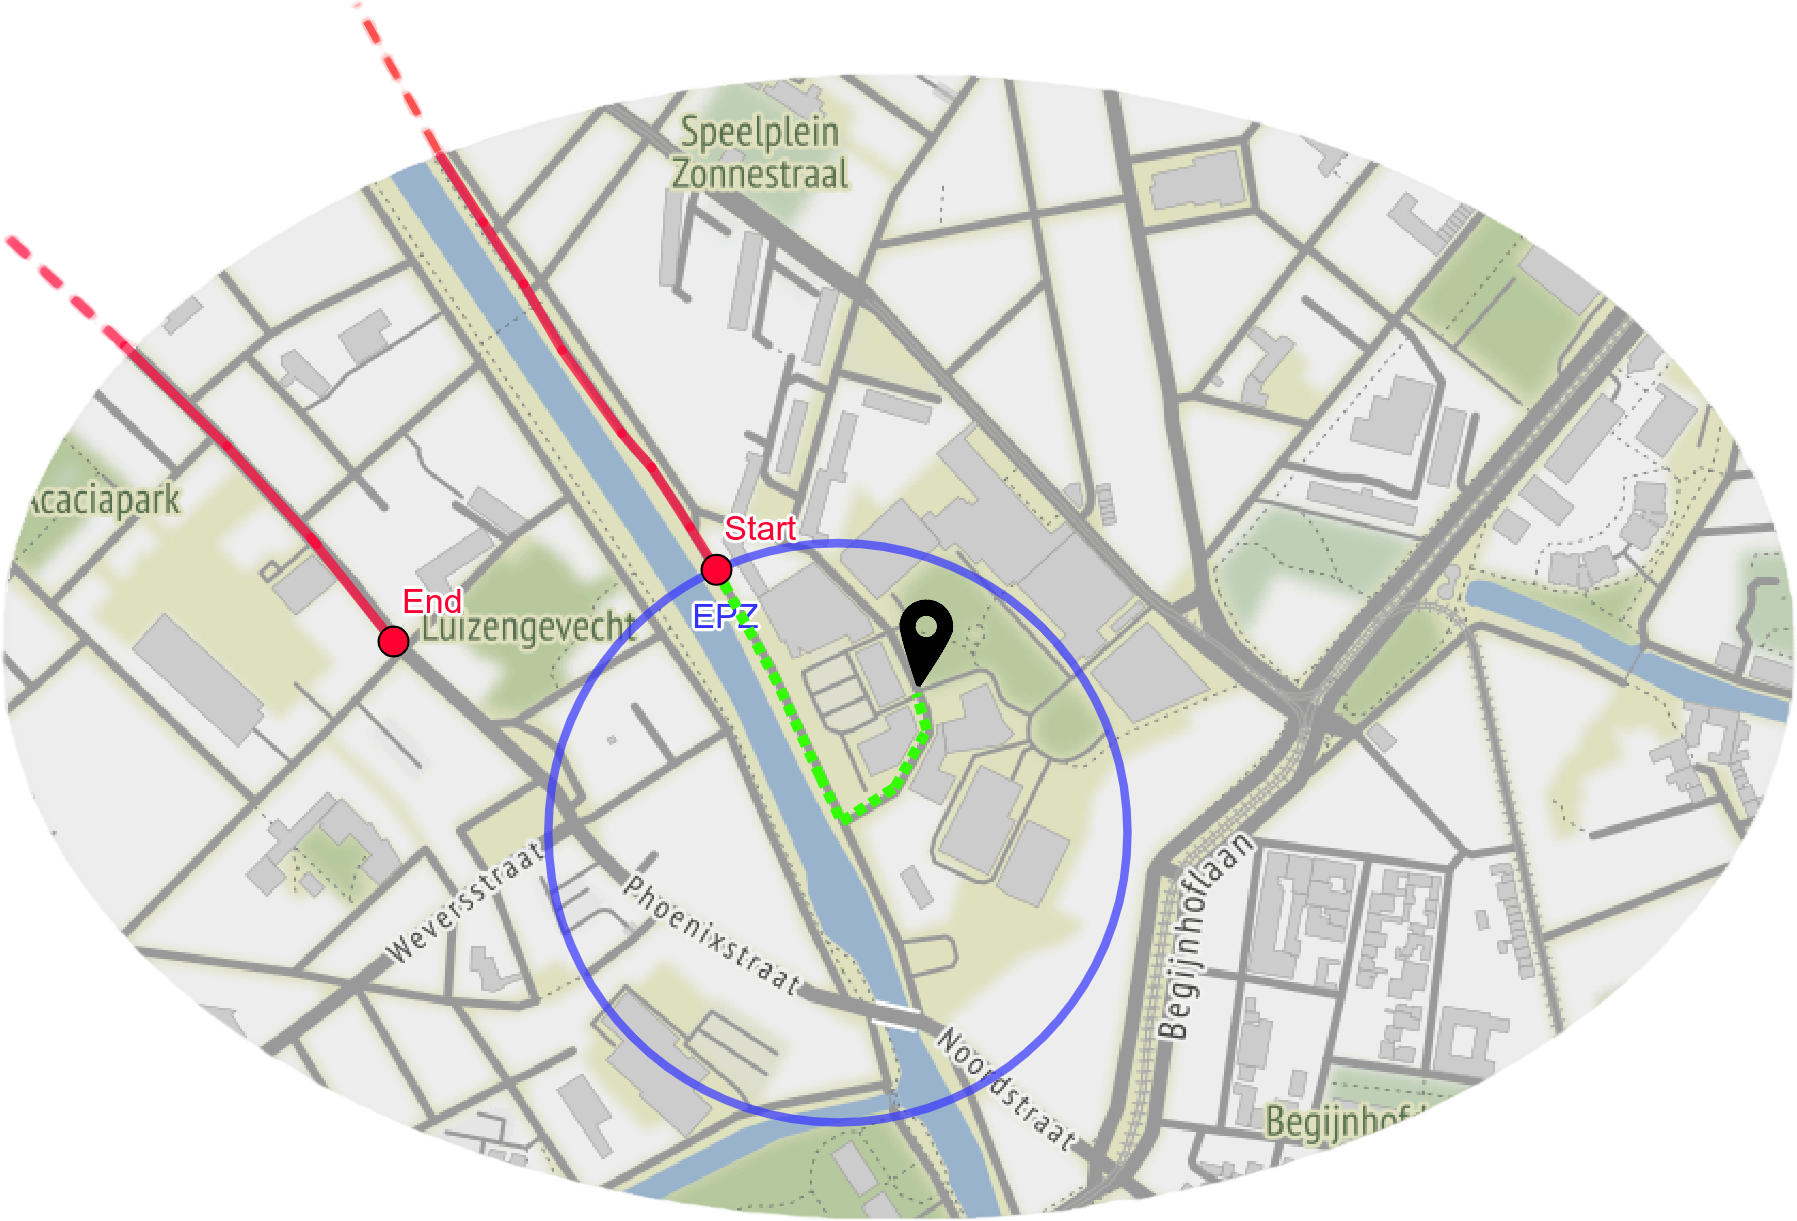
\includegraphics[width=1\textwidth]{fig/TotalDistanceAttacks/start.png}
    \end{subfigure}\hfill
    \begin{subfigure}[b]{.5\textwidth}
        \centering
        \caption{Einde binnenin de \ac{EPZ}}
        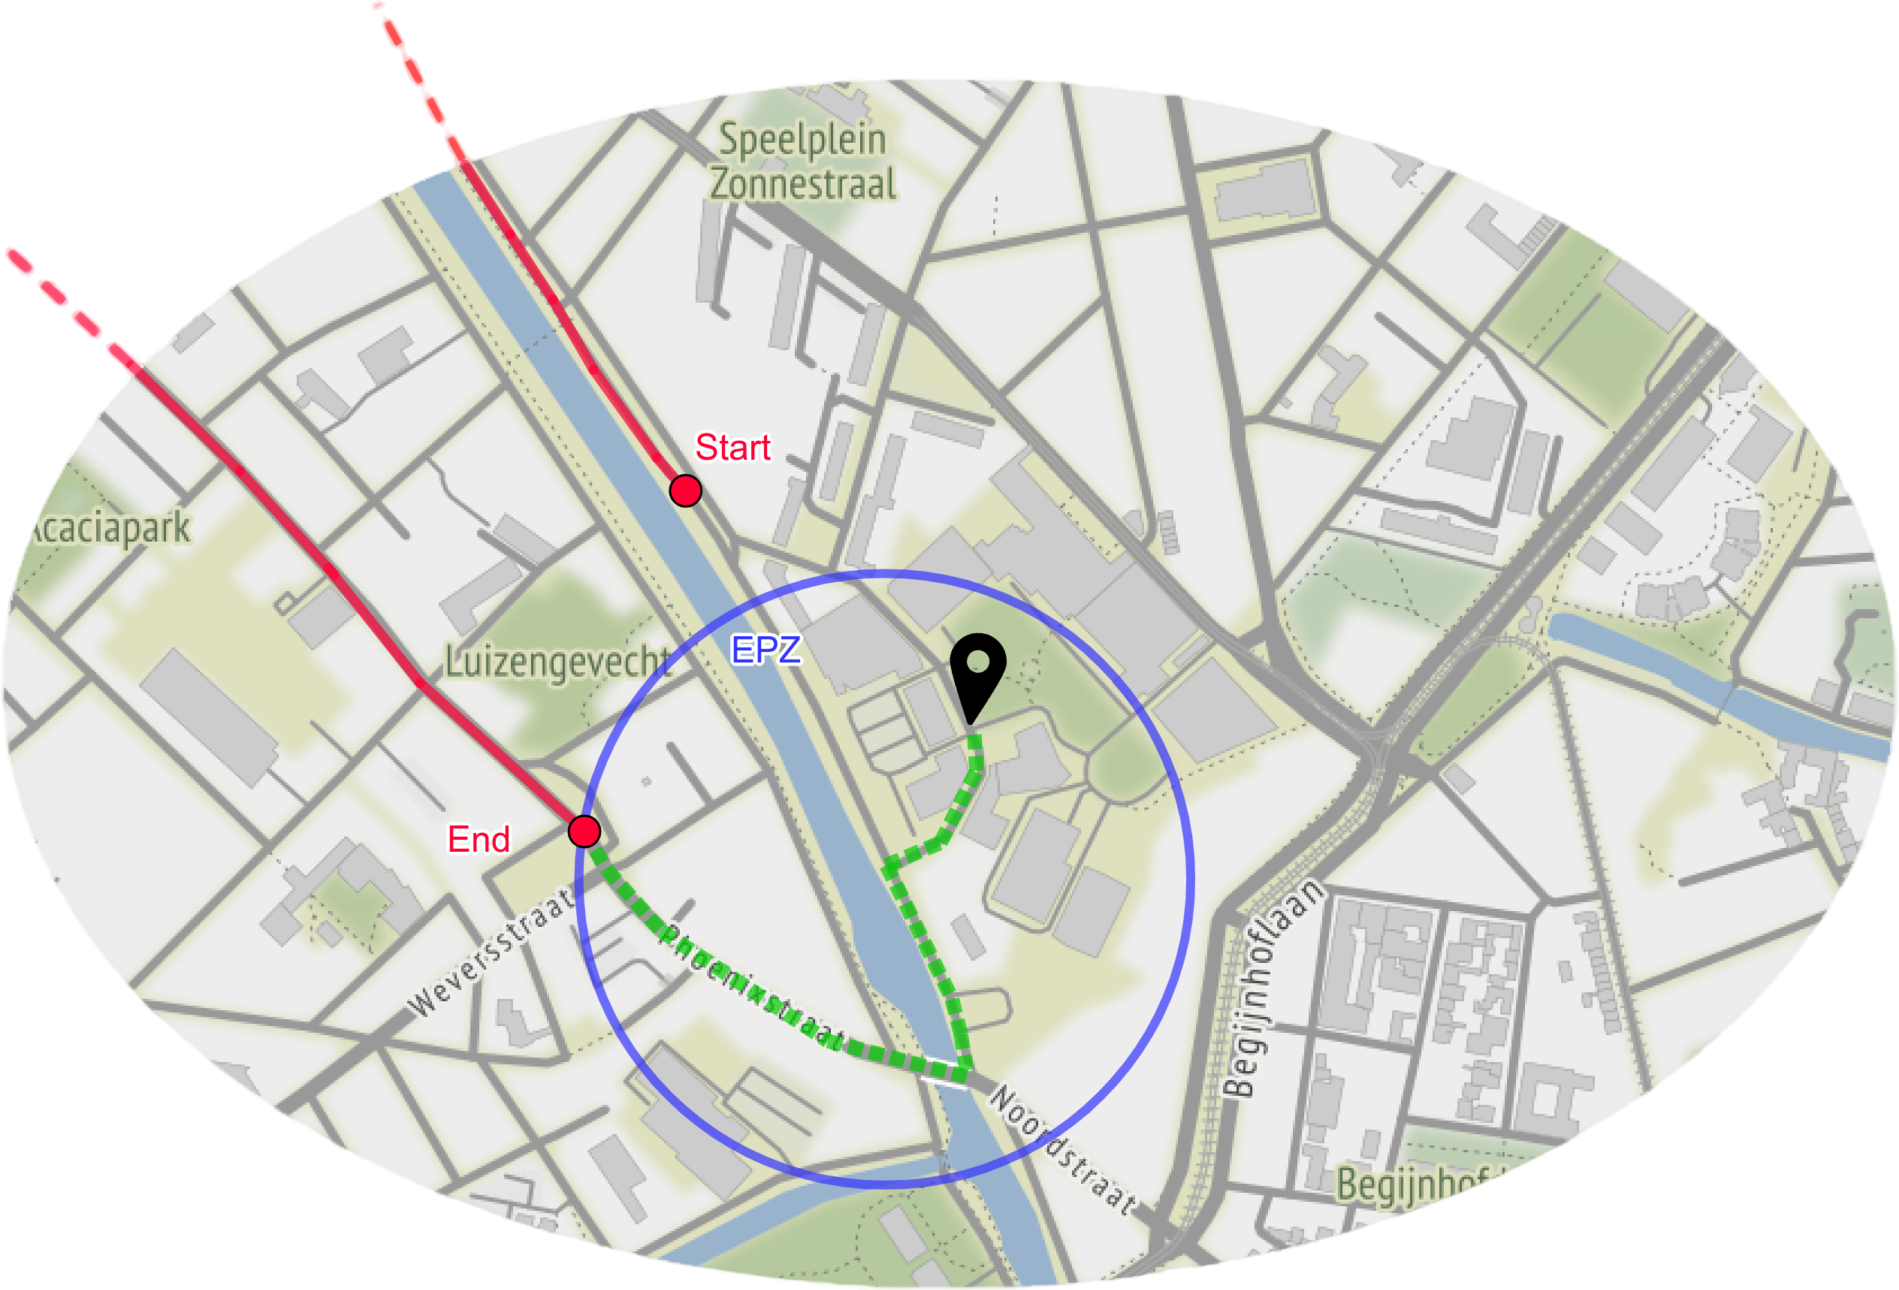
\includegraphics[width=1\textwidth]{fig/TotalDistanceAttacks/end.png}
    \end{subfigure}
    \caption{Voorbeeld van de mogelijke scenarios bij een total distance attack scenario}\label{fig:totalDistanceAttack}
\end{figure}
\begin{figure}[h]
    \centering
    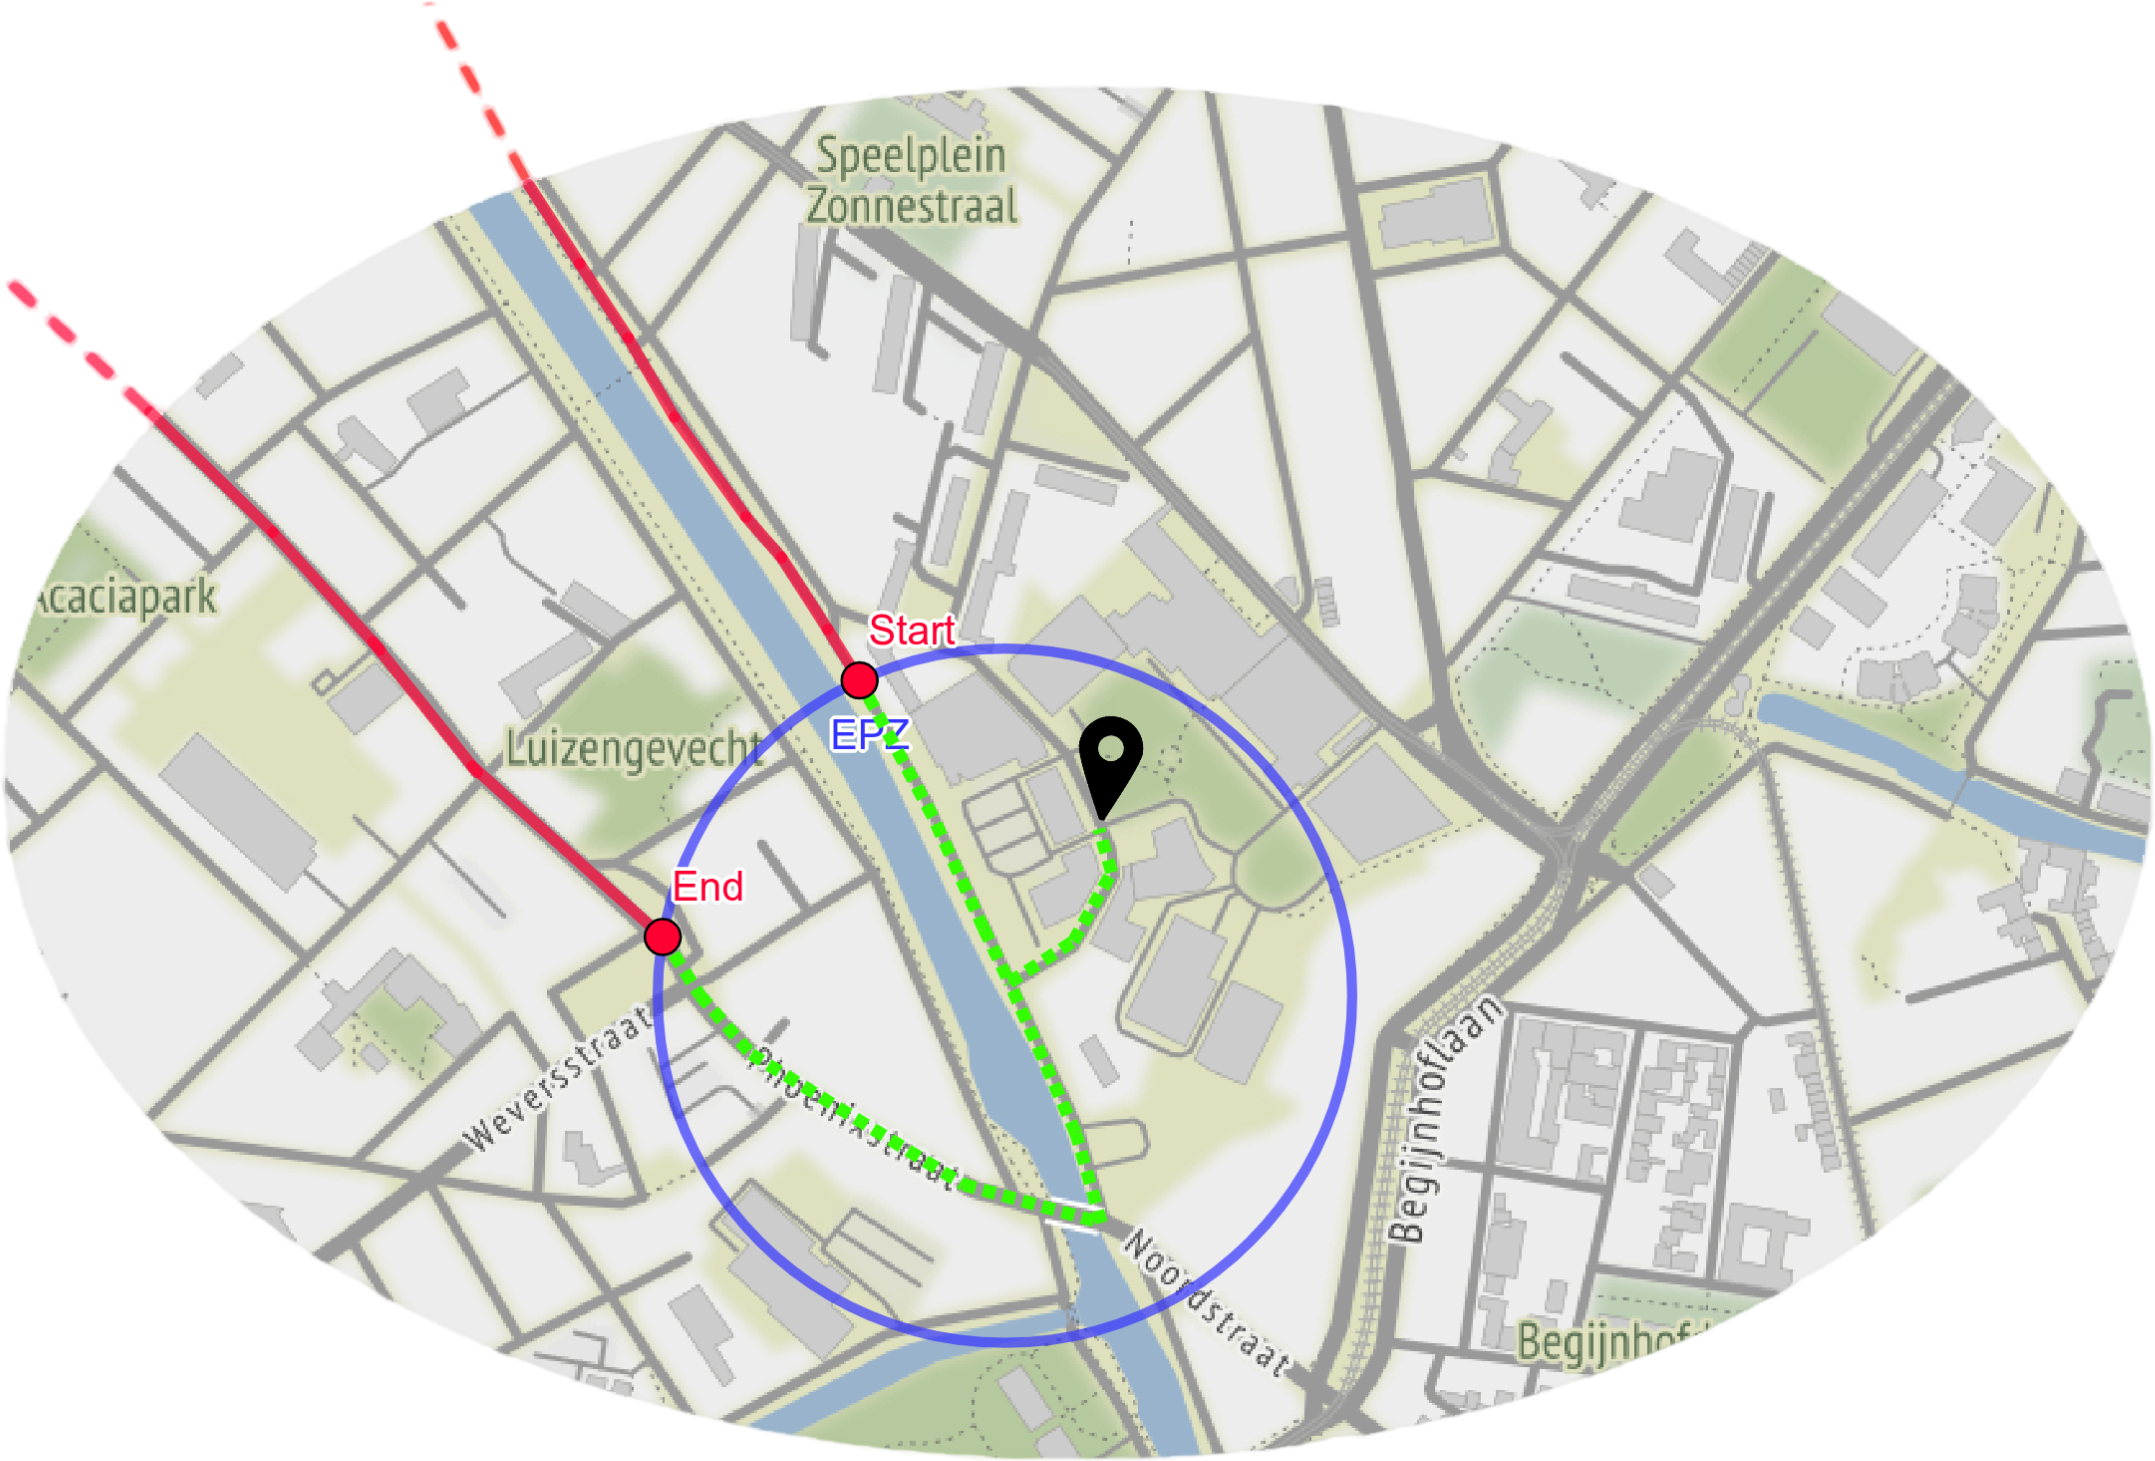
\includegraphics[width=.5\textwidth]{fig/TotalDistanceAttacks/InnerDistanceAttack.png}
    \caption{Voorbeeld van een inner distance attack situatie}\label{fig:innerDist}
\end{figure}

Deze thesis baseert zich ook voor een stuk op gemiddelde snelheden en tempo's.
Hierdoor stellen we volgende bijkomende assumptie voor: een gebruiker mag niet
stilstaan binnenin de \ac{EPZ}. Platformen zoals Strava hebben namelijk een
ingebouwde functie die bij het uploaden van een activiteit tijdstippen waarbij
een gebruiker stilstaat aan bijvoorbeeld een rood licht filtert. De gebruikers
hebben op deze manier een representatievere gemiddelde snelheid en gemiddeld
tempo. Dit wil wel zeggen dat de totale bewegingstijd waarop de gemiddelde
snelheid en tempo gebaseerd zijn, niet overeenkomt met de totale tijd van de
activiteit. Bij een berekening gebaseerd op totale verstreken tijd zou een
significante fout kunnen optreden.
% Momenteel zijn op de meeste platformen beide
% tijden afzonderlijk gegeven, maar in het theoretisch kader van dit onderzoek
% lijkt het ook nuttig om te testen in hoeverre de aanval succesvol is indien gene 

\section{Identificeren van de EPZ}
De eerste stap is het identificeren van de \ac{EPZ}. Alhoewel deze stap niet
noodzakelijk is, vernauwt deze de zoekruimte drastisch. Hierbij nemen we van
alle activiteiten die van een gebruiker ter beschikking zijn gesteld, de
zichtbare begin- en eindpunten genomen. Deze zullen dan via het k-means
algoritme worden gegroepeerd en een cirkel vormen.

K-means clustering is een unsupervised machine learning techniek die veel wordt
gebruikt bij het clusteren van data. Het is een iteratief proces waarbij het
algoritme $k$ clusters tracht te creëren waarbij de datapunten in elke cluster
zo dicht mogelijk bij het gemiddelde van die cluster
liggen~\cite{Understa24:online}. Dit algoritme kiest willekeurig initiële
middelpunten voor de verschillende clusters. Daarna kent het alle punten in de
data toe aan de cluster met de laagste Euclidische afstand tot het centrum van
deze cluster. Daarna herberekent het algoritme de gemiddeldes van deze
clusters, en worden deze gemiddeldes gezien als nieuwe centrums. Opnieuw zal
het alle punten aan de correcte cluster toekennen, en het proces herhaald zich
verschillende iteraties op deze manier. Op Figuur~\ref{fig:kmeans} is te zien
hoe de clustering bij elke iteratie beter wordt.
\begin{figure}[h]
    \centering
    \begin{subfigure}[b]{.33\textwidth}
        \centering
        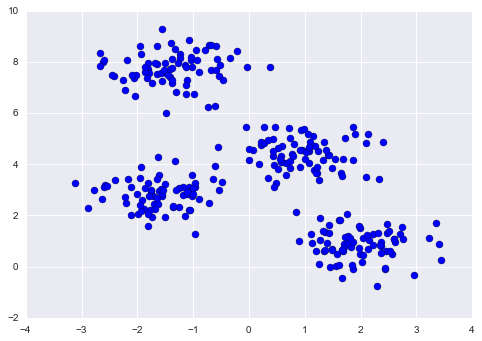
\includegraphics[width=1\textwidth]{fig/kmeans/1.png}
    \end{subfigure}\hfill
    \begin{subfigure}[b]{.33\textwidth}
        \centering
        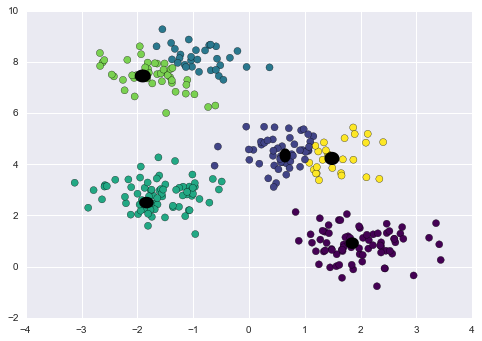
\includegraphics[width=1\textwidth]{fig/kmeans/2.png}
    \end{subfigure}
    \begin{subfigure}[b]{.33\textwidth}
        \centering
        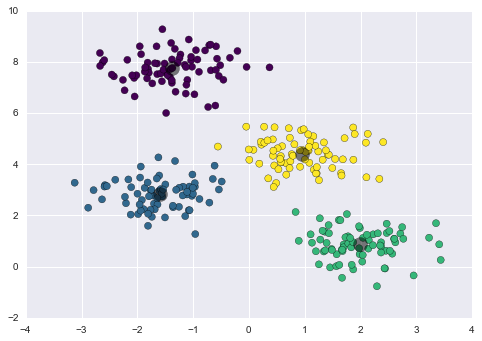
\includegraphics[width=1\textwidth]{fig/kmeans/3.png}
    \end{subfigure}
    \caption{Voorbeeld werking k-means clustering~\cite{InDepthk59:online}}\label{fig:kmeans}
\end{figure}

In de context van het identificeren van de \ac{EPZ} gebruiken we k-means om
\ac{gps}-punten te groeperen op basis van hun locaties. In plaats van te werken
met een centraal punt, werkt onze implementatie met een cirkelvormige zone, wat
zichtbaar is op Figuur~\ref{fig:kmeans_circle}. De euclidische afstand zullen
we in dit geval berekenen ten opzichte van de rand van deze cirkel. Bij elke
iteratie beschouwen we een nieuwe cirkel, en berekenen we de afstanden opnieuw.
We herhalen het proces totdat een stabiele cirkel bekomen wordt. Een cirkel is
stabiel wanneer het verschil in afstand tussen twee opeenvolgende gevonden
cirkels kleiner is dan een drempelwaarde, in dit geval 10 meter~\cite{Dhondt,
    Verdonck_2022}.
\begin{figure}[h]
    \centering
    \begin{subfigure}[b]{0.49\linewidth}
        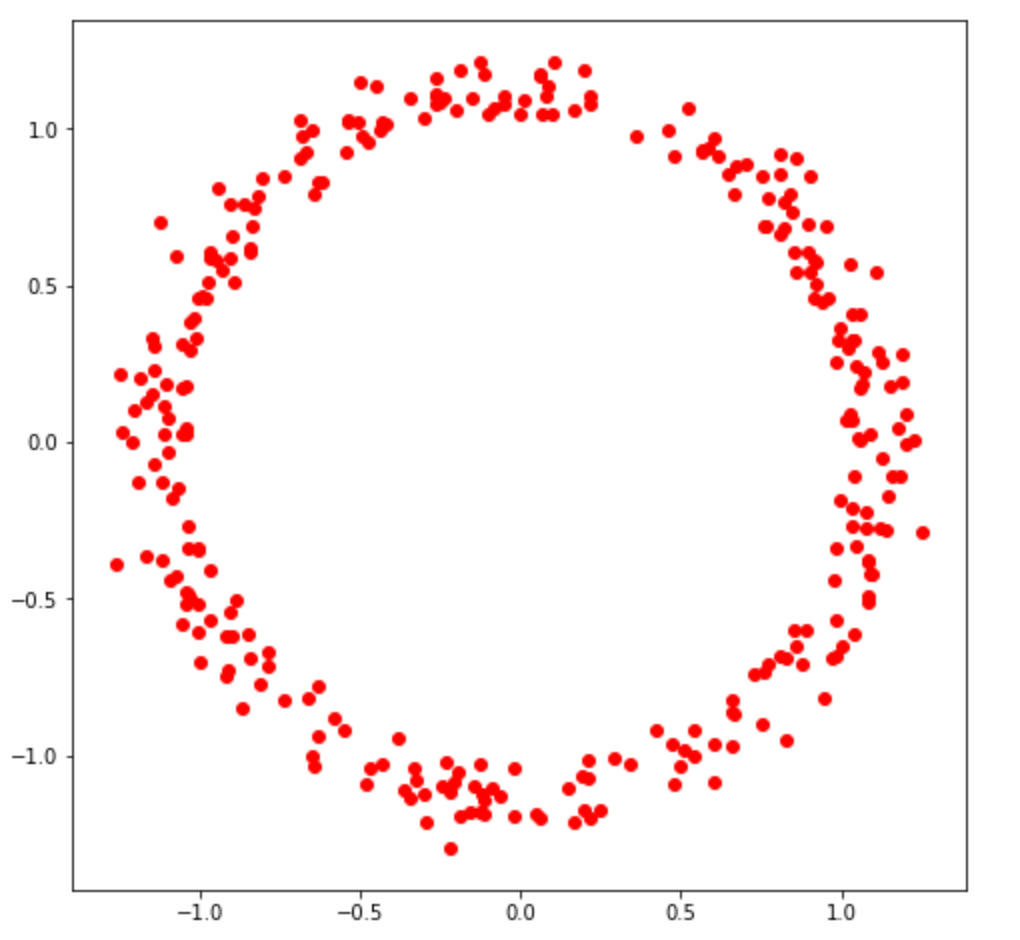
\includegraphics[width=\linewidth]{fig/kmeans/kmeans_circle.png}
    \end{subfigure}
    \begin{subfigure}[b]{0.49\linewidth}
        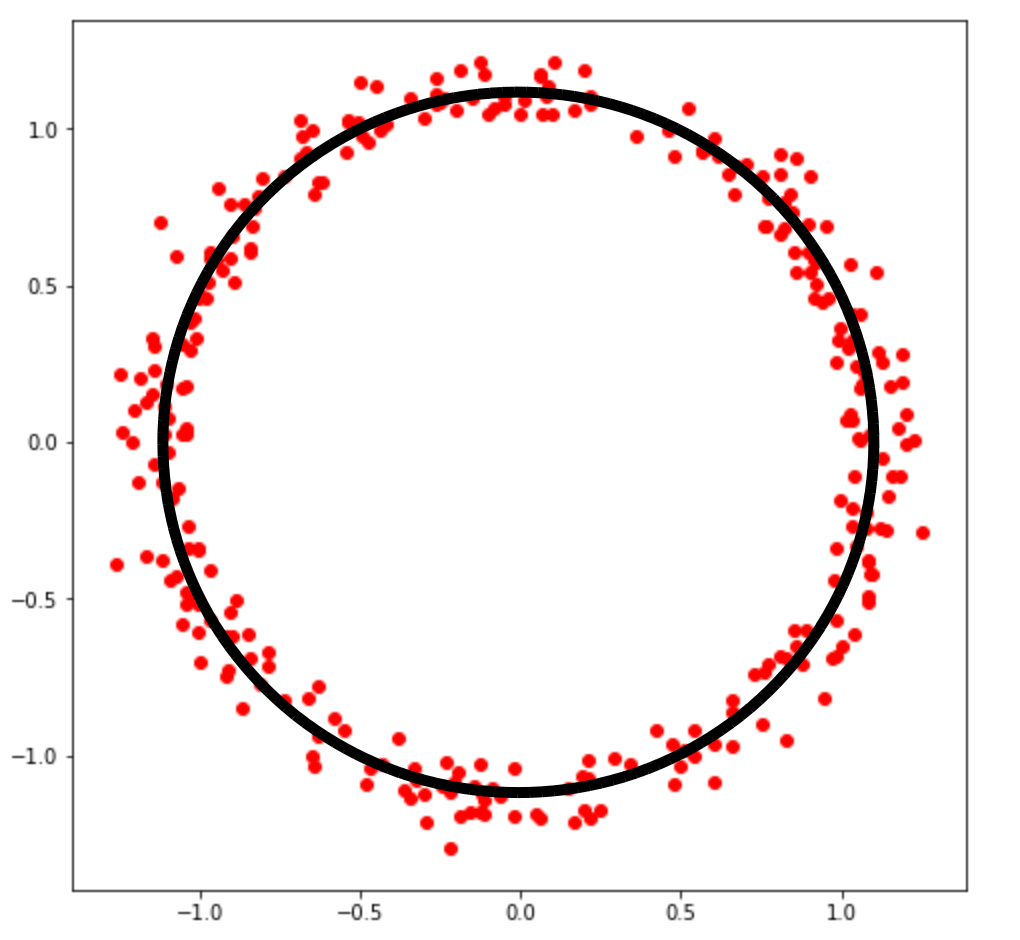
\includegraphics[width=\linewidth]{fig/kmeans/kmeans_circle copy.png}
    \end{subfigure}
    \caption{Example of datapoints which can identify a circle~\cite{DensityE3:online}}\label{fig:kmeans_circle}
\end{figure}

Het algoritme zal na de identificatie van een \ac{EPZ} ook nog nakijken of er
niet meer dan één \ac{EPZ} te vinden is. Het onderzoekt of punten die
meegenomen zijn in de beschouwing van de huidige \ac{EPZ}, toch niet horen bij
een mogelijks andere \ac{EPZ} van de user. Als controle berekent het van elk
eind- of beginpunt de Euclidische afstand tot de rand van de bijhorende
gevonden \ac{EPZ}. Indien deze kleiner is dan de grootst mogelijke radius, dan
veronderstellen we dat het punt bij deze zone hoort. Indien dit voor alle
punten geldt, dan stopt het algoritme hier. In het andere geval waarbij de
berekende afstand groter is, worden meer clusters toegevoegd aan het algoritme
van k-means clustering. Dit zal dus een nieuwe privacy zone aanwijzen.

Deze stap is niet noodzakelijk in het globale verhaal van de thesis, maar is
wel een stap die de zoekruimte drastisch kan verkleinen. Indien het algoritme
één of meerdere \acp{EPZ} vindt, dan zullen er enkel en alleen voorspellingen
gebeuren in de regio binnenin de geïdentificeerde zone. Indien dit niet het
geval is en er geen \ac{EPZ} gevonden is, bestaat de kans dat voorspellingen
van locaties gebeuren buiten de verhullende zone. Ook is in dit geval een
groter stuk van het stratennetwerk nodig om de locatie te achterhalen.

\section{Identificatie Entry Gates}
Entry gates zijn zoals de naam al doet vermoeden de `toegangspoorten' tot de
\ac{EPZ}. Dit zijn de `zones' waar de gebruiker de \ac{EPZ} kan betreden en/of
verlaten. Deze vormen zich dan ook rond wegen die de \ac{EPZ} betreden. Op
Figuur~\ref{fig:entrygate} is te zien dat meerdere eindpunten van activiteiten
geclusterd worden en een \ac{E.G.} vormen. Dit is van belang belangrijk bij het
filteren van afwijkende activiteiten. De detectie ervan gebeurt via het
\ac{DBSCAN}-algoritme.
\begin{figure}
    \centering
    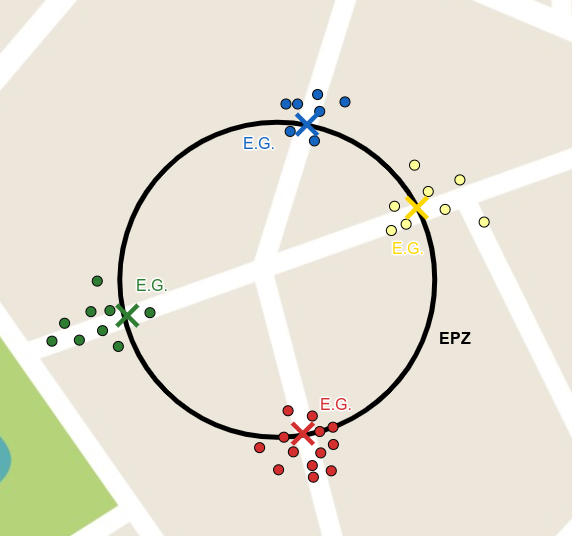
\includegraphics[width=0.5\linewidth]{fig/EPZ-mechanisme/Entry_Gate.png}
    \caption{Voorbeeld van entry gates gevonden door k-means clustering en de identificatie van een EPZ}\label{fig:entrygate}
\end{figure}

\ac{DBSCAN} is een algoritme dat clusters kan vinden in een dataset. Het vindt
clusters op basis van hun dichtheid~\cite{KMeansvs80:online}. In tegenstelling tot het eerder besproken
k-means clustering algoritme dat gebaseerd is
op het vinden van de geometrische centra van clusters, richt \ac{DBSCAN}
zich op het vinden van gebieden met een hoge dichtheid van punten.\ \ac{DBSCAN}
heeft als voordeel dat het goed overweg kan met uitschieters, want in deze
context erg nuttig blijkt. Het werkt als volgt:
\begin{enumerate}
    \item Selecteer een willekeurig niet-bezocht punt uit de set van zichtbare begin- en
          eindpunten.
    \item Bepaal of het punt een kernpunt is door te controleren of er binnen een
          bepaalde afstand een minimum aantal punten aanwezig is. Als dit het geval is,
          wordt het punt als een kernpunt beschouwd en wordt een nieuwe cluster gestart.
    \item Breid de cluster uit door alle punten binnen deze afstand van het kernpunt toe
          te voegen aan de cluster. Herhaal dit proces voor alle punten in de buurt
          totdat er geen nieuwe punten meer kunnen worden toegevoegd.
    \item Ga door naar het volgende niet-bezochte punt en herhaal de stappen 2 en 3
          totdat alle punten in de dataset zijn bezocht.
    \item Punten die niet tot een cluster behoren en niet voldoen aan de criteria voor
          kernpunten, worden beschouwd als ruispunten.
\end{enumerate}
Het algoritme maakt gebruik van twee op voorhand vast te leggen parameters: de maximale afstand tussen twee
punten in eenzelfde cluster, wat in deze context vastgelegd is op 22.9 meter en
een minimaal aantal punten dat de cluster moet bevatten, in dit geval één punt.

\section{Bepalen nodige gegevens voor predictie}
Na het bepalen van de \acp{EPZ} van de gebruiker gaan we over tot het berekenen
en achterhalen van de bijhorende gegevens die nodig zijn om de gevoelige
locatie te voorspellen. Hiervoor wordt verder ingegaan op de methodiek
beschreven inferentieaanval door~\citeauthor{Dhondt}, maar er worden enkele
gegevens op een andere manier benaderd volgens de huidige definitie van de
aanvaller.

\subsection{Roadgraph en Distance Matrix}\label{sec:roadgraph}
Voor elke gevonden EPZ is het noodzakelijk om een graafvoorstelling van de
omgeving op te stellen. Op Figuur~\ref{fig:graph_generation} is een voorbeeld
terug te vinden van hoe een graaf kan worden geëxtraheerd. Er worden punten
geplaatst op de straten op een vaste afstand van
elkaar\footnote{\label{fn:roadgraph}Op de Figuur~\ref{fig:graph_generation}
    zijn de afstanden niet altijd gelijk. De figuur is enkel nuttig ter
    illustratie, en is geen perfecte representatie de werkelijkheid.}, en deze
kunnen dan worden verbonden. Indien geen \acp{EPZ} geïdentificeerd zijn, nemen
we een ruime omgeving die we omzetten naar een graaf. De graafvoorstelling
bestaat uit een serie van nodes, die zich allemaal op een gekende straat
bevinden. De bogen waarmee de nodes verbonden zijn volgen het straatplan, opdat
een boog een mogelijks te volgen weg is~\cite{neira2022graph}. Aan de hand van
de `Chaining Distance' wordt bepaald hoeveel afstand tussen de nodes zal
zitten, en zo dus impliciet ook welke densiteit het netwerk zal hebben. Hoe
lager de chaining distance, hoe meer nodes, en dus ook hoe preciezer de
graafvoorstelling zal zijn. Om voorspellingen te maken is wel een bepaalde
precisie vereist, dus mag deze waarde niet te hoog zijn. Empirisch koos
\citeauthor{Dhondt} voor een waarde van $3.0$ meter.
\begin{figure}[h]
    \caption{Voorbeeld van het genereren van een roadgraph\footref{fn:roadgraph}}\label{fig:graph_generation}
    \centering
    \begin{subfigure}[b]{.4\textwidth}
        \centering
        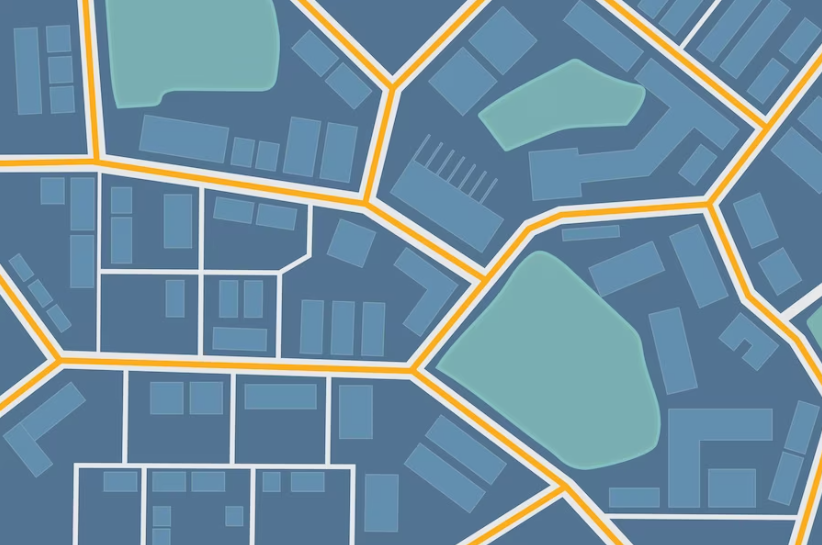
\includegraphics[width=1\textwidth]{fig/RoadGraph/RoadMap.png}
        \caption{Voorbeeld stratenplan}
    \end{subfigure}\hfill
    \begin{subfigure}[b]{.4\textwidth}
        \centering
        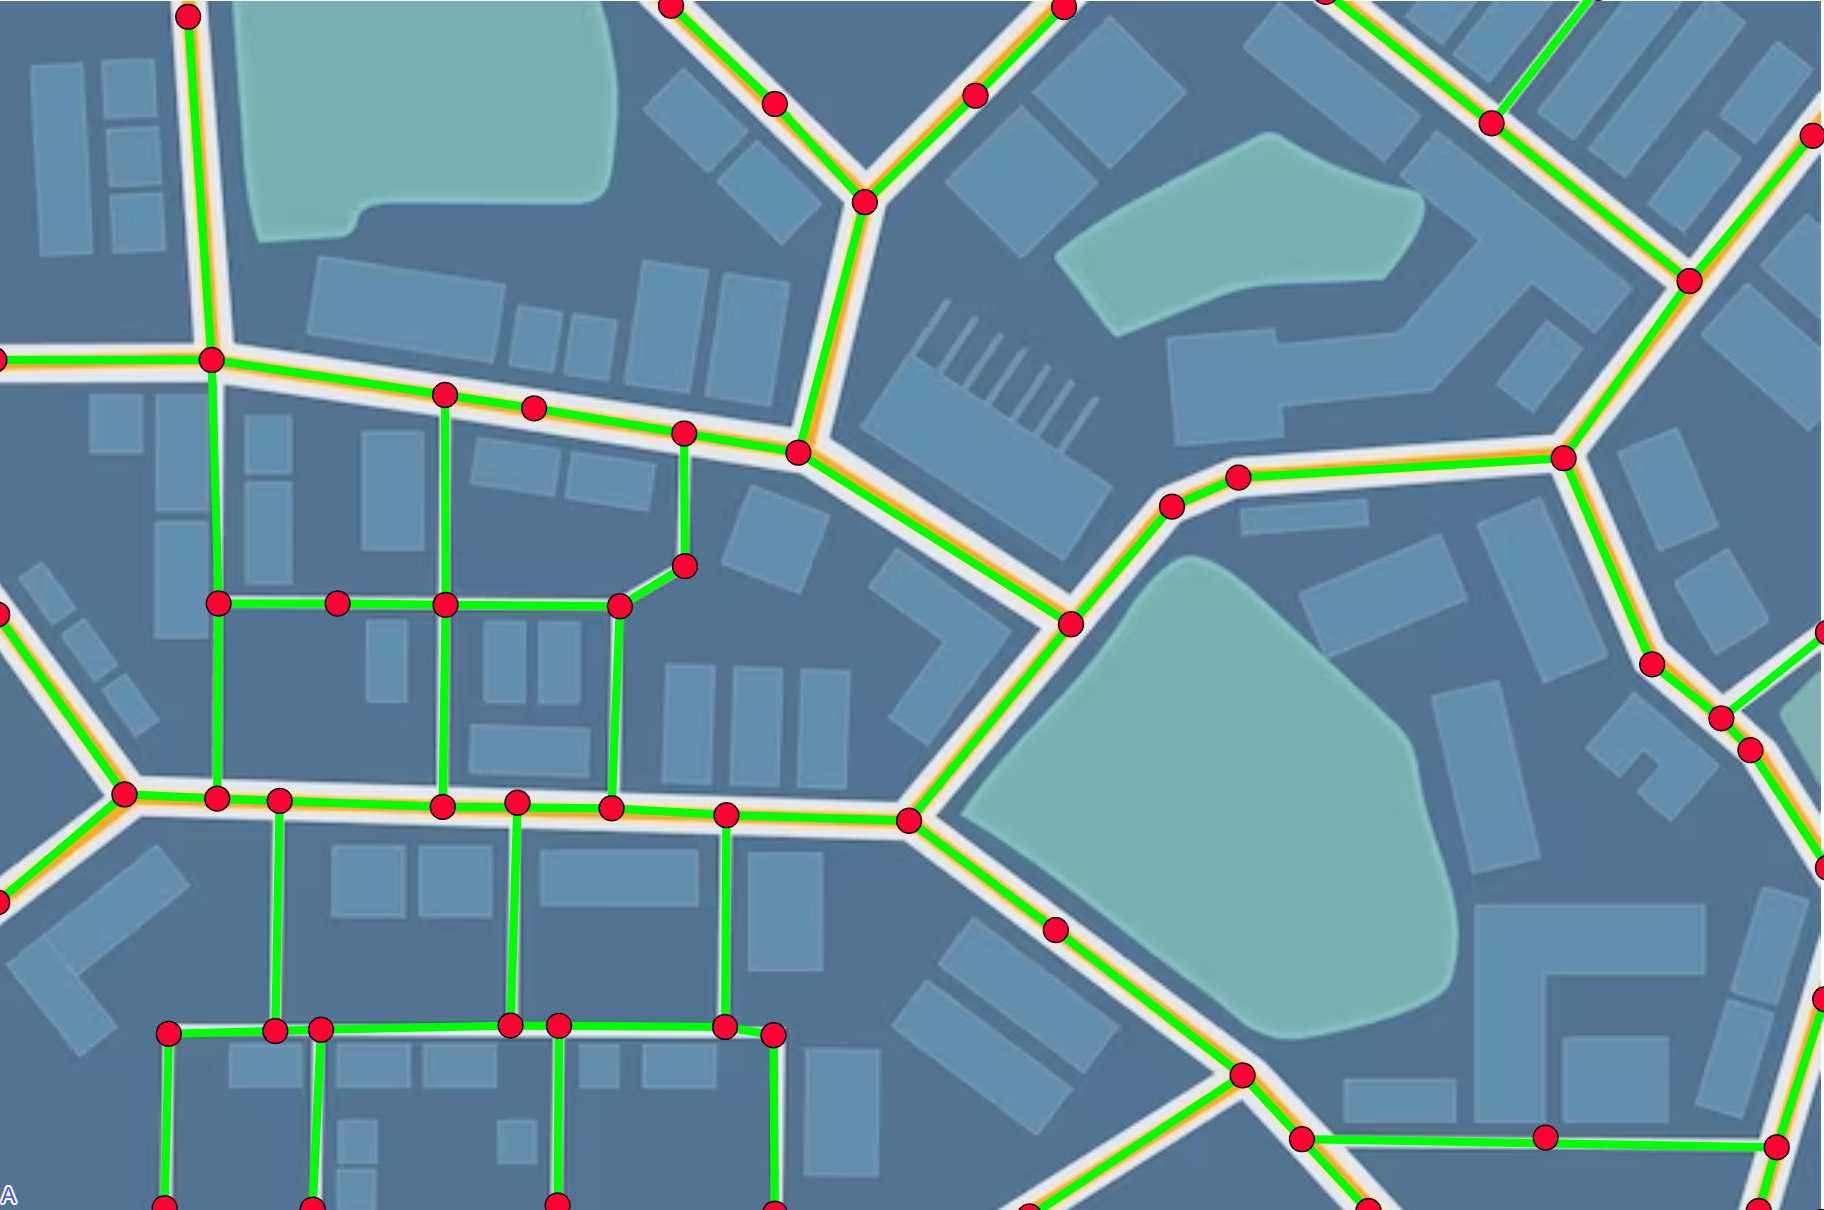
\includegraphics[width=1\textwidth]{fig/RoadGraph/Graph_Over_Map.png}
        \caption{Nodes en bogen geplot op het stratenplan}
    \end{subfigure}
    \begin{subfigure}[b]{.4\textwidth}
        \centering
        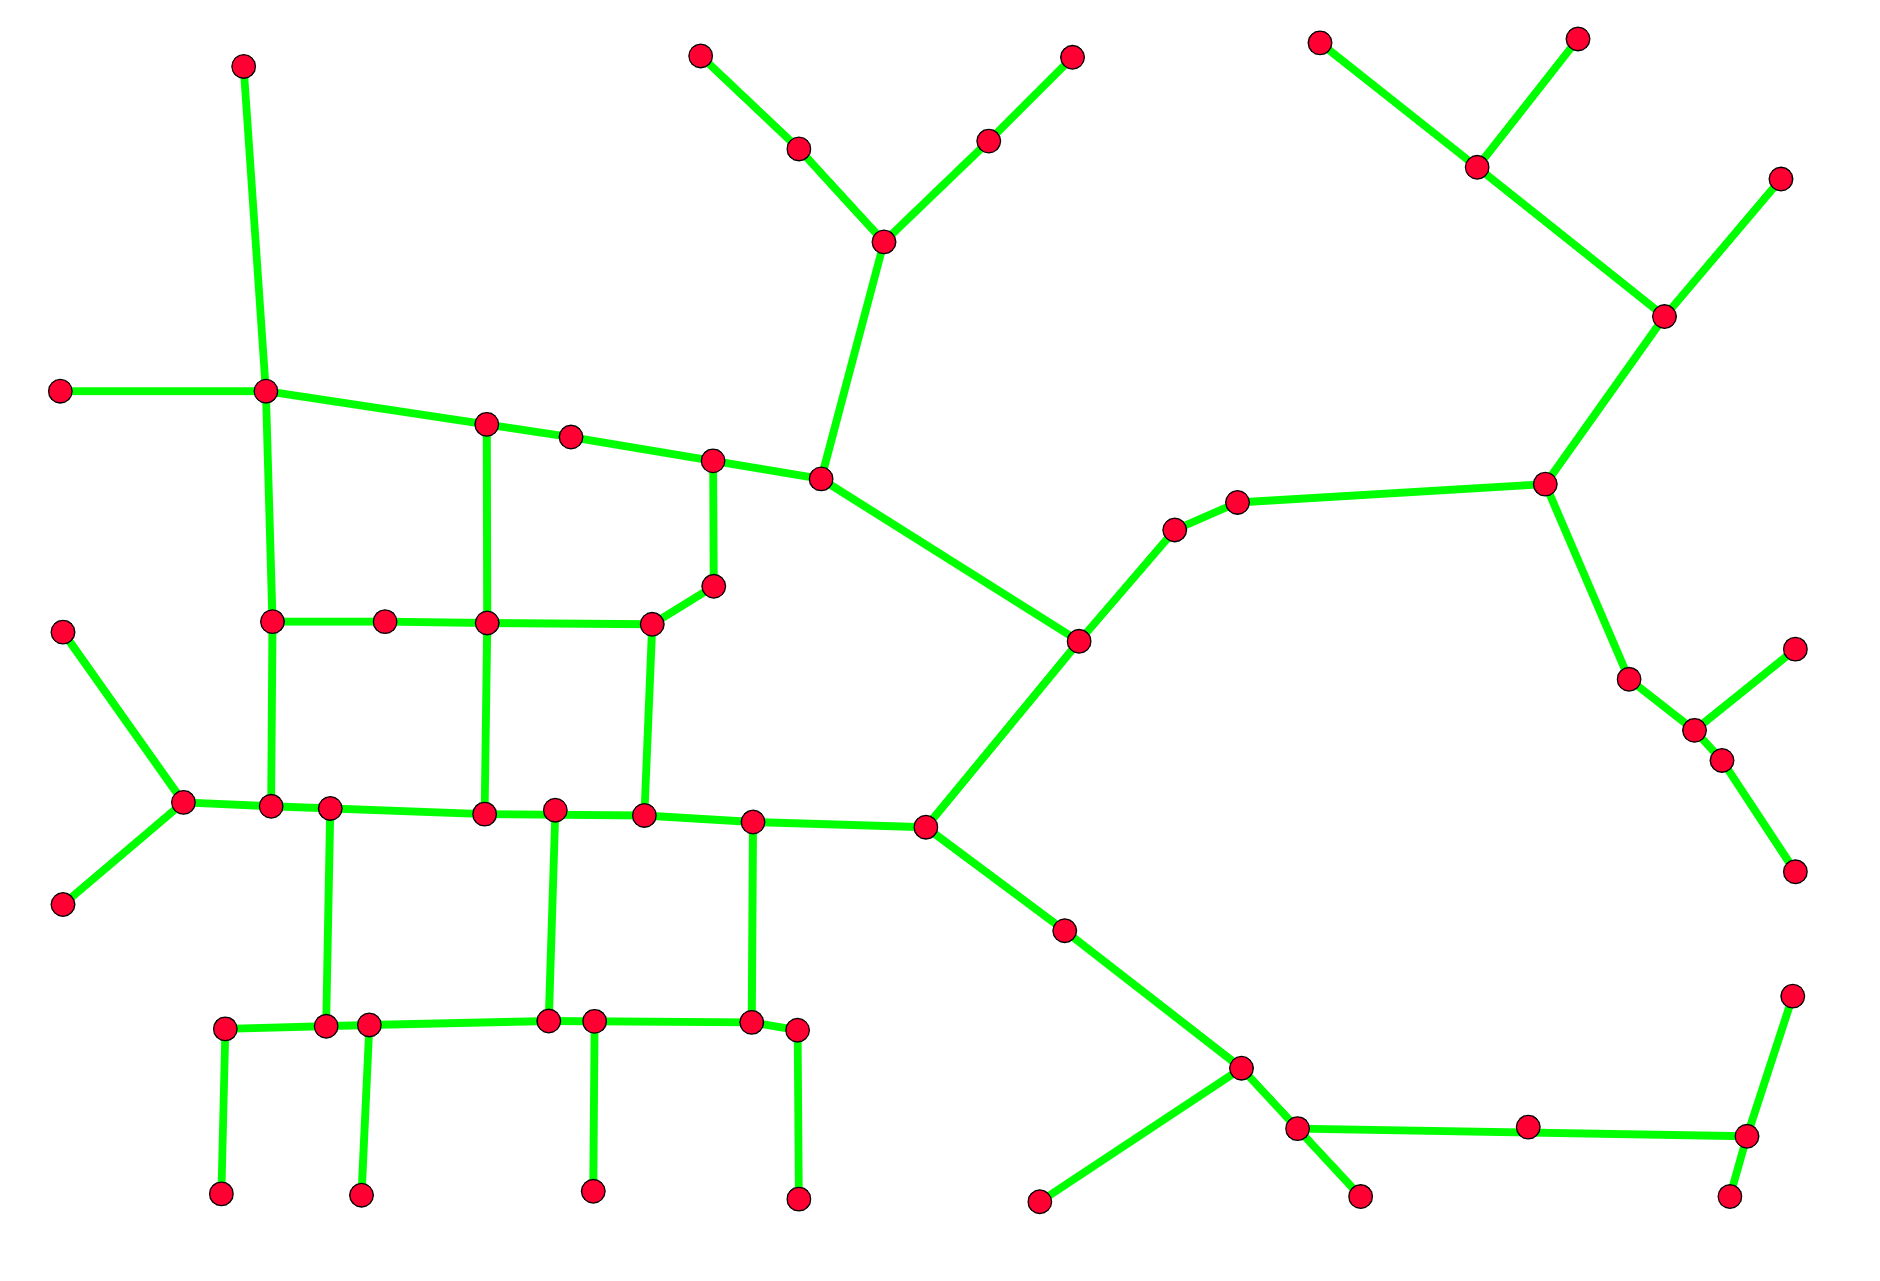
\includegraphics[width=1\textwidth]{fig/RoadGraph/Graph.png}
        \caption{Resulterende graafvoorstelling van het stratenplan}
    \end{subfigure}
\end{figure}

Op basis van de nodes in deze graaf, kan de \textit{Distance Matrix} worden
opgesteld. Dit is een matrix die voor alle startnodes (op de rand van de
\ac{EPZ}) de theoretische afstand bevat tot alle nodes aanwezig in de graaf.
Gebruikmakend van het Dijkstra algoritme\footnote{Het Dijkstra-algoritme is een
    algoritme in de grafentheorie dat wordt gebruikt om de kortste weg te vinden
    tussen twee knooppunten in een gewogen grafiek~\cite{dijkstra}. Het algoritme
    werkt door iteratief knooppunten toe te voegen aan een `bezochte' set en de
    kortste afstand te berekenen vanaf het beginpunt naar elk aangrenzend knooppunt
    dat nog niet is bezocht.}, die het in staat stelt om voor elk punt de kortste
theoretische afstand te bepalen tot alle punten in de graaf. Deze afstanden
worden opgeslagen, en zijn belangrijk in een verder stadium van de aanval.

\subsection{Begin- en eindnodes}
Voor elke activiteit is het volledige traject buiten de \ac{EPZ} gegeven. Dit
omvat alle \ac{gps}-punten die niet verborgen zijn. De begin- en eindnodes van
het traject zijn hier van belang. Voor de duidelijkheid en de vlotheid van de
tekst zullen we naar deze punten refereren als het zichtbare beginpunt en het
zichtbare eindpunt. Volgens één van de voorafgaand gemaakt assumptie vertrekt
de sporter in de \ac{EPZ} of eindigt hij erbinnen, maar beide is geen
mogelijkheid. Dit betekent dat ofwel het reële eindpunt, ofwel het reële
beginpunt zal overeenstemmen met de gevoelige locatie. In geval dat een
gebruiker aankomt binnenin de \ac{EPZ}, en dus ook vertrekt erbuiten, starten
de berekeningen vanaf het zichtbare eindpunt. Omgekeerd geldt indien de
gebruiker vertrekt binnenin de \ac{EPZ}, worden de berekeningen gestart vanaf
het zichtbare beginpunt. Deze punten zullen in het vervolg \textit{randpunten}
genoemd worden, refererend naar de rand van de \ac{EPZ}. Deze randpunten zullen
de basis vormen voor de volgende berekeningen.

Bijhorend zijn bij de randpunten ook bepaalde extra gegevens beschikbaar. De
belangrijkste zijn de cumulatieve afstand tot dit punt\footnote{De totale
    afstand afgelegd vanaf het begin van de activiteit tot en met het punt in
    kwestie.}, en de cumulatieve tijd tot dit punt\footnote{De totale tijd afgelegd
    vanaf het begin van de activiteit tot en met het punt in kwestie.}. Bij de
aanval van Dhondt et al.\ wordt de afstand gebruikt om predicties te doen. Dit
wil dus zeggen dat deze afstand dus aan de basis zal liggen. In deze thesis
wordt ervan uitgegaan dat afstanden verborgen worden. Onder het verbergen van
afstanden wordt een onderscheid gemaakt tussen 2 scenarios: het eerste gaat
ervan uit dat de totale afstand verborgen wordt, maar de cumulatieve afstand
gegeven is. Het tweede scenario gaat ervan uit dat alle afstandsgegevens
verborgen worden. Het alternatieve type data waar dus mee zal moeten gewerkt
worden is dus \ac{gps}-data.

\subsection{Berekeningen afstand binnenin de EPZ}\label{sec:berekeningen}
Om voorspellingen te kunnen doen zullen volgens de inferentieaanval die we hier
bespreken, moeten twee belangrijke gegevens ter beschikking zijn. Met name het
straatnetwerk met de mogelijks gevolgde routes, wat werd besproken in
Sectie~\ref{sec:roadgraph}, en de afstand die wordt afgelegd binnenin de
\ac{EPZ}. Deze afstand benoemen we ook als de \textit{inner distance} (dit is
niet te verwarren met de \textit{inner ditstance attack}).

In de implementatie van~\citeauthor{Dhondt} kan de \textit{inner distance}
simpelweg berekend worden door het verschil te nemen tussen de afgelegde
afstand buiten de verhulde zone (deze noemen we de \textit{outer distance}), en
de totale afstand: \[inner\ distance = total\
    distance - outer\ distance \]

In deze thesis is er echter een tussenstap noodzakelijk. In het eerste scenario
waarbij de cumulatieve afstand gegeven is, maar de totale afstand niet, moet de
totale afstand berekend worden. Maar door de aanwezigheid van snelheids- en
tijdsgegevens kan dit via basisformules gebeuren. Gebruik makend van het
gemiddelde tempo kan de voorgaande formule worden omgevormd tot: \[inner\ distance = total\ time \times average\ speed - outer\ distance \]

In opzicht van het tweede scenario, waarbij alle afstandsgegevens verborgen
zijn, ontbreekt nu ook de \textit{outer distance}. We bepalen deze via de
\ac{gps}-coördinaten. Dit gebeurd door de som te nemen van de afstanden van
tussen alle opeenvolgende punten. Let wel dat we de afstand tussen twee
\ac{gps}-punten berekenen door gebruik te maken van de \textit{haversine}
formule. Vergelijking~\ref{eq:haversine} is een uitwerking van deze
formule~\cite{sheppard1922practical}. Deze berekent de afstand tussen twee
punten op een bolvormig oppervlak, in dit geval de aarde. De breedte- en
lengtegraden van elk punt moeten omgezet worden naar radialen. Vervolgens
worden deze waarden ingevoerd in de formule, samen met de straal van de aarde
($r$), meestal genomen als $6.371 km$. De formule berekent dan de haversine
($haversine(\theta)=\sin^2(\frac{\theta}{2})$) van de helft van het verschil
tussen de breedtegraden en de haversine van de helft van het verschil tussen de
lengtegraden ($\lambda$), evenals de cosinus van de breedtegraden ($\phi$) van
beide punten. Deze waarden worden vervolgens gebruikt om de afstand tussen de
twee punten (P \& Q op Figuur~\ref{fig:haversine}) te berekenen.

Merk op dat ook dit een benadering is van de werkelijke afstand. De aarde is
niet perfect sferisch, wat de nauwkeurigheid kan beïnvloeden. Maar voor de
doeleinden binnen deze thesis is dit voldoende nauwkeurig, zeker omdat de
afstanden in deze context relatief klein zijn, waardoor over het algemeen
slechts een minimale buiging is.
\begin{equation}\label{eq:haversine}
    d = 2r \arcsin\left(\sqrt{\sin^2\left(\frac{\phi_2-\phi_1}{2}\right)+\cos(\phi_1)\cos(\phi_2)\sin^2\left(\frac{\lambda_2-\lambda_1}{2}\right)}\right)
\end{equation}
\begin{figure}[h]
    \centering
    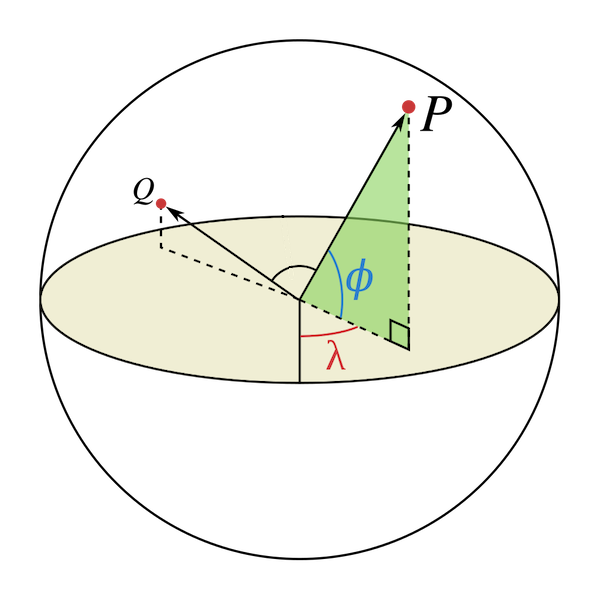
\includegraphics[width=0.5\textwidth]{fig/haversine.png}
    \caption{Haversine illustratie voor het berekenen van de afstand~\cite{Distance97:online}}\label{fig:haversine}
\end{figure}

Uit de voorgaande paragrafen kunnen we dus besluiten dat de inner distance af
te leiden valt uit gegeven outer distance, total time en de gemiddelde
snelheid. Om een \textit{outer distance attack} uit te voeren is de berekening
van de totale inner distance voldoende. Maar bij het uitvoeren van een
\textit{inner distance attack} zijn de twee afzonderlijke inner distances nodig
(degene van start tot de \ac{EPZ} en degene van de \ac{EPZ} tot de finish).
Wanneer de cumulatieve afstand gegeven is, zouden we een deze aanval kunnen
uitvoeren doordat in dit geval de twee afstanden te achterhalen zijn.
$d_{start} = d_{eerste\ node}$ en $d_{finish} = d_{totaal} - d_{laatste\
            node}$. Maar wanneer deze niet beschikbaar zijn, is dit niet mogelijk, in dit
geval zijn deze afstanden niet individueel te achterhalen.

\section{Voorspellen locatie}
Alle nodige gegevens zijn nu beschikbaar om de gevoelige locatie te
achterhalen. Hier wordt besproken hoe voor elke bruikbare activiteit een
locatie zal worden voorspeld. Doordat voor elke activiteit één of meerdere
locaties worden voorspeld, zullen we deze moeten bundelen tot één locatie voor
alle activiteiten.

\subsection{Filteren activiteiten}
Voorafgaand aan het voorspellen is het van essentieel belang om uitsluitend
voorspellingen te maken op basis van activiteiten die een waardevolle
voorspelling kunnen genereren. Andere activiteiten zouden enkel de accuraatheid
van de voorspelling naar beneden halen. Dit gaat dan bijvoorbeeld over
activiteiten waarbij niet de kortste route binnenin de \ac{EPZ} wordt gevolgd.
Al deze activiteiten proberen we dus in de mate van het mogelijke eruit te
filteren.

Het geval waarbij een gebruiker niet de kortste route volgt vanaf de rand van
de \ac{EPZ} tot de gevoelige locatie kunnen we in zekere mate opvangen door te
stellen dat we een activiteit enkel nog gebruiken wanneer de nog af te leggen
afstand binnenin de \ac{EPZ} kleiner is dan de maximaal mogelijk af te leggen
weg. In de andere gevallen zullen we de activiteit weggooien. De maximale
afstand die hiervoor nodig is wordt bepaald gebruik makend van de
\textit{Distance Matrix}, die beschreven staat in Sectie~\ref{sec:roadgraph}.
De maximale afstand is gelijk aan de maximale afstand terug te vinden in de
matrix, voor de bijhorende startnode. Dit is de afstand die een gebruiker
maximaal kan afleggen naar eender welke node op de graaf, vertrekkend van de
startnode, door het volgen van de theoretisch kortste route. Dit zal ook
gevallen in rekening brengen waarbij het traject voor een stuk verborgen wordt,
maar niet zal eindigen op de gevoelige locatie.

Op een gelijkaardige manier kan een filtering gebeuren voor afgelegde afstanden
die lager zijn dan de minimale mogelijke afstand. Dit zou opnieuw activiteiten
kunnen filteren die niet eindigen op de gevoelige afstand. De minimale afstand
is dan ook degene tot de node met de laagste minimale afstand tot deze node
vanaf het zichtbare startpunt of eindpunt van de activiteit, gelegen op de rand
van de \ac{EPZ}.

Om de zichtbare eind- en beginpunten van de activiteiten te controleren op
compatibiliteit met de road graph, voeren we een actieve verificatie uit.
Hierbij worden alle eind- en beginpunten op de graaf `gesnapt', ofwel vervangen
door de dichtstbijzijnde knooppunt op de graaf. We berekenen de afstand tussen
de oorspronkelijke locatie en de gesnapte locatie. Indien het verschil in
afstand te groot is, filteren we de betreffende activiteit. Een aanzienlijk
verschil in afstand kan duiden op een afwijking tussen de gevolgde route en de
road graph, of op onnauwkeurige gps-gegevens.

Als laatste wordt nog gekeken naar afwijkingen bij de \acp{E.G.}. Indien bij
een activiteit een afwijking wordt vastgesteld tussen de zichtbare begin- en
eindpunten en de \ac{E.G.} die groter is dan drie maal de standaardafwijking,
wordt de activiteit gefilterd. Dit wijst dan op een te grote spreiding bij ten
opzichte van de \ac{E.G.}, en dus op een grote kans op inaccurate
voorspellingen.

\subsection{Bepalen van de locatie}
Om een predictie te maken per activiteit wordt de inner distance die berekend
werd in Sectie~\ref{sec:berekeningen} gebruikt. Deze wordt dan gematched met
het stratennetwerk. Het idee hierachter is om alle mogelijke routes (die de
kortste route vormt naar alle nodes op zijn pad) binnenin de \ac{EPZ} af te
leggen, en te stoppen wanneer de afgelegde afstand gelijk is aan de berekende
inner distance. Het resultaat van deze gevolgde route is dan een node, die
mogelijks de gevoelige locatie kan voorstellen. In de praktijk kunnen we dit
mechanisme op een simpele manier toepassen door gebruik te maken van de vooraf
berekende distance matrix. De berekende inner distance zal worden vergeleken
met de afstanden in de distance matrix.

Deze methodiek herhalen we voor elke activiteit die niet werd gefilterd. Al
deze voorspellingen worden uiteindelijk gebundeld tot één voorspelling in de
volgende stap.

\subsection{Regressie om te komen tot een eindvoorspelling}\label{sec:lad}
Om de routes die we in vorige sectie bepaalden om te vormen tot één
eindvoorspelling, voeren we een regressie-analyse uit, aan de hand van de
\ac{LAD} methode. Het resultaat van deze regressie-analyse zal een
\ac{gps}-locatie zijn, die onze \textit{eindvoorspelling} zal vormen.

De \ac{LAD} methode wordt gebruikt om een lineaire regressie uit te voeren op
een set punten, door de som van de absolute waarden van de absolute verschillen
te minimaliseren.\ \ac{LAD} staat gekend als een robuuste methode die erg
nuttig blijkt te zijn voor datasets met grote uitschieters. In
Vergelijking~\ref{eq:LAD} is te zien dat, door het werken met absolute waarden,
extremen in mindere mate doorwegen in de berekeningen. Dit is een groot
voordeel ten opzichte van andere regressietechnieken, zoals
bijvoorbeeld~\ac{OLS}~\cite{iqbal2021application}.~\ac{OLS} werkt gelijkaardig,
maar zoals te zien is in Vergelijking~\ref{eq:OLS} probeert deze de som van de
kwadratische afwijkingen te minimaliseren. Uitschieters zullen dus meer
doorwegen. Een nadeel van \ac{LAD} is dat het berekenen van de LAD-schattingen
meer rekentijd en computerbronnen vereist dan \ac{OLS}, wat het minder geschikt
maakt voor grote datasets.
\begin{equation} \label{eq:LAD}
    LAD:\indent  \min\sum\limits_{i=1}^n|d_i - d_{inner}|
\end{equation}
\begin{equation} \label{eq:OLS}
    OLS:\indent  \min\sum\limits_{i=1}^n{(d_i - d_{inner})}^2
\end{equation}

In deze context gebruiken we LAD regressie door de aard van de data en
voorspellingen, meer bepaald door de grote kans op uitschieters. Gps-data kan
erg onnauwkeurig zijn, en grote of kleine afwijkingen kunnen dus voorkomen. Ook
is het mogelijk dat door acties van een sporter zoals bijvoorbeeld eenmalig de
kortste route niet volgen, uitschieters voorvallen. Rekentijd is in deze thesis
geen probleem, aangezien de dataset beperkt blijft tot 100 activiteiten.

In de context van deze thesis kan Vergelijking~\ref{eq:LAD} worden toegepast
voor elke node in de graaf. Elke node in graaf zullen we individueel beschouwen
als een mogelijke eindvoorspelling. Het verschil tussen de nog af te leggen
afstand voor deze activiteit, of dus de inner distance en de theoretische
afstand tot de node vanaf het zichtbare begin- of eindpunt, wat af te lezen
valt uit de distance matrix, stelt dan de afwijking voor van deze activiteit.
Indien we dit sommeren over alle activiteiten voor dezelfde node, bekomen we
een waarde die de totale afwijking voorstelt indien we voor deze node als
eindvoorspelling zouden kiezen. We overlopen alle nodes in de graaf, en
selecteren deze met de laagste totale afwijking. Deze node zal dan de
\textbf{eindvoorspelling} voor deze activiteit voorstellen.

% Alle voorspelde locaties zullen worden beschouwd als mogelijke
% \textit{eindvoorspelling}. Deze zal dan in de vergelijking $\hat{y}$
% voorstellen. De absolute waarde van het verschil tussen de eindvoorspelling en
% alle overige punten zal worden opgeteld. Er wordt gezocht naar het punt waarbij
% de som van de absolute waarde minimaal is, en dit is dan de resulterende
% predictie, de \textbf{eindvoorspelling}.
%%%%%%%%%%%%%%%%%%%%%%%%%%%%%%%%%%%%%%%%%%%%%%%%%%%%%%%%%%%%%%%%%%% 
%                                                                 %
%                            CHAPTER                              %
%                                                                 %
%%%%%%%%%%%%%%%%%%%%%%%%%%%%%%%%%%%%%%%%%%%%%%%%%%%%%%%%%%%%%%%%%%% 
\chapter{Gebruikte data en afwijkingen}
De aanval die beschreven werd in Hoofdstuk~\ref{chap:inferentieaanval} testen
we op groep aantal gebruikers met hun desbetreffende activiteiten, om zo
zinvolle conclusies te trekken over de vatbaarheid van gebruikers op
fitnessplatformen voor deze aanval. Maar het is dan ook essentieel dat een
correcte dataset wordt gebruikt, en dat de eigenschappen die deze dataset heeft
worden beschreven. We onderzoeken eigenschappen en mogelijke afwijkingen of
onregelmatigheden opdat een gefundeerde conclusie kan worden gevormd, die
eventueel bepaalde eigenschappen van de dataset mee in rekening brengt.

Aangezien deze thesis voor een stuk verder bouwt op het onderzoek
van~\citeauthor{Dhondt_Pochat_Voulimeneas_Joosen_Volckaert_2022}, is het
evident om verder te werken op deze
dataset~\cite{Dhondt_Pochat_Voulimeneas_Joosen_Volckaert_2022}. Deze dataset
werd volledig zelf gescraped vanaf de officiële \ac{API} van het platform
`Strava'\footnote{\url{https://www.strava.com/}}. De scope van deze dataset is
een periode van één week, startend op 11 juli 2021 00:00 \ac{UTC}. De site werd
chronologisch afgelopen en voor alle activiteiten, met sprongen van 9000
activiteiten. Let wel dat door mogelijke vertragingen door bijvoorbeeld het
uploaden van een activiteit, de activiteiten niet exact chronologisch kunnen
worden opgehaald. Indien een activiteit privaat is of gecloaked\footnote{Een
    gecloakede activiteit is een activiteit waar al een EPZ op is aangebracht.
    Aangezien deze thesis uncloaked activities nodig heeft~\ref{sec:zelf_cloaking}
    zijn ze dus niet bruikbaar. Men kan zien of een activiteit gecloaked is indien
    er een verschil is tussen de zichtbare afstand en de totale afstand.} is, of
reeds verwijdert is, dan zal deze worden overgeslagen en de volgende worden
genomen. Voor elke activiteit die succesvol werd gevonden, wordt daarna de
gebruiker beschouwd. Van alle bekomen gebruikers worden dan de rest van de
activiteiten afgehaald en bijgehouden in één grote dataset. De gegevens worden
ook geanonimiseerd opgeslagen, zodat de gebruikers niet meer kunnen worden
geïdentificeerd. De dataset bevat dus geen namen of andere persoonlijke
gegevens, enkel ID's.

In totaal werd een dataset van 4000 gebruikers verzameld. Deze thesis
experimenteert echter slechts met een subset van 131 users, waarvan er 101
gebruikt worden voor analyses en conclusies, en 30 voor het testen van de
aanval.

\section{Karakteristieken van de gebruikte dataset}
Op Figuur~\ref{fig:geographic_spread} is de geografische spreiding van de
activiteiten gevisualiseerd aan de hand van een heatmap. Hierop is duidelijk te
zien dat de meeste activiteiten zich in Centraal-Europa bevinden. Daarnaast is
ook een duidelijke concentratie te zien in de Verenigde Staten. In mindere mate
zijn ook activiteiten in Australië en Zuid-Amerika. De dataset bevat dus
relatief een grote spreiding van activiteiten over de hele wereld, wat een
goede basis is voor het testen van de aanval. Let wel, de dataset is met 101
gebruikers echter wel relatief klein, wat een vertekend beeld kan geven van de
werkelijkheid.

Op Tabel~\ref{tab:stats_dataset} zijn enkele globale statistieken met
betrekking tot gebruikers en de bijhorende activiteiten van de dataset
weergegeven. Er valt op dat de dataset per gebruiker toch meestal een groot
aantal activiteiten ter beschikking zijn. De gemiddelde gebruiker bevat 411
activiteiten, de mediaan is 296. Volgens de inferentieaanval beschreven in
Hoofdstuk~\ref{chap:inferentieaanval} resulteert een gebruiker met meer
activiteiten over het algemeen in een accuratere aanval. Op
Figuur~\ref{fig:cdf_amount_activities} is de \ac{CDF} plot\footnote{Een
    Cumulative Distribution Function (CDF) plot is een grafiek die de cumulatieve
    verdeling van de waarden van een continue variabele
    weergeeft~\cite{CursusSt38:online}. De x-as van de grafiek bevat de
    verschillende waarden die de continue variabele kan aannemen, terwijl de y-as
    de kans aangeeft dat de variabele een waarde kleiner dan of gelijk aan die op
    de x-as aanneemt. De curve van de CDF laat zien hoe waarschijnlijk het is dat
    een willekeurige waarde van de continue variabele kleiner is dan een bepaalde
    drempelwaarde.} te zien die het aantal activiteiten per gebruiker weergeeft.
Hierop worden voorgaande besluiten enkel maar bevestigd. Het plot duidt ook aan
dat meer dan 20\% van de gebruikers een aantal activiteiten heeft dat groter is
dan 100.

\begin{figure}[h]
    \centering
    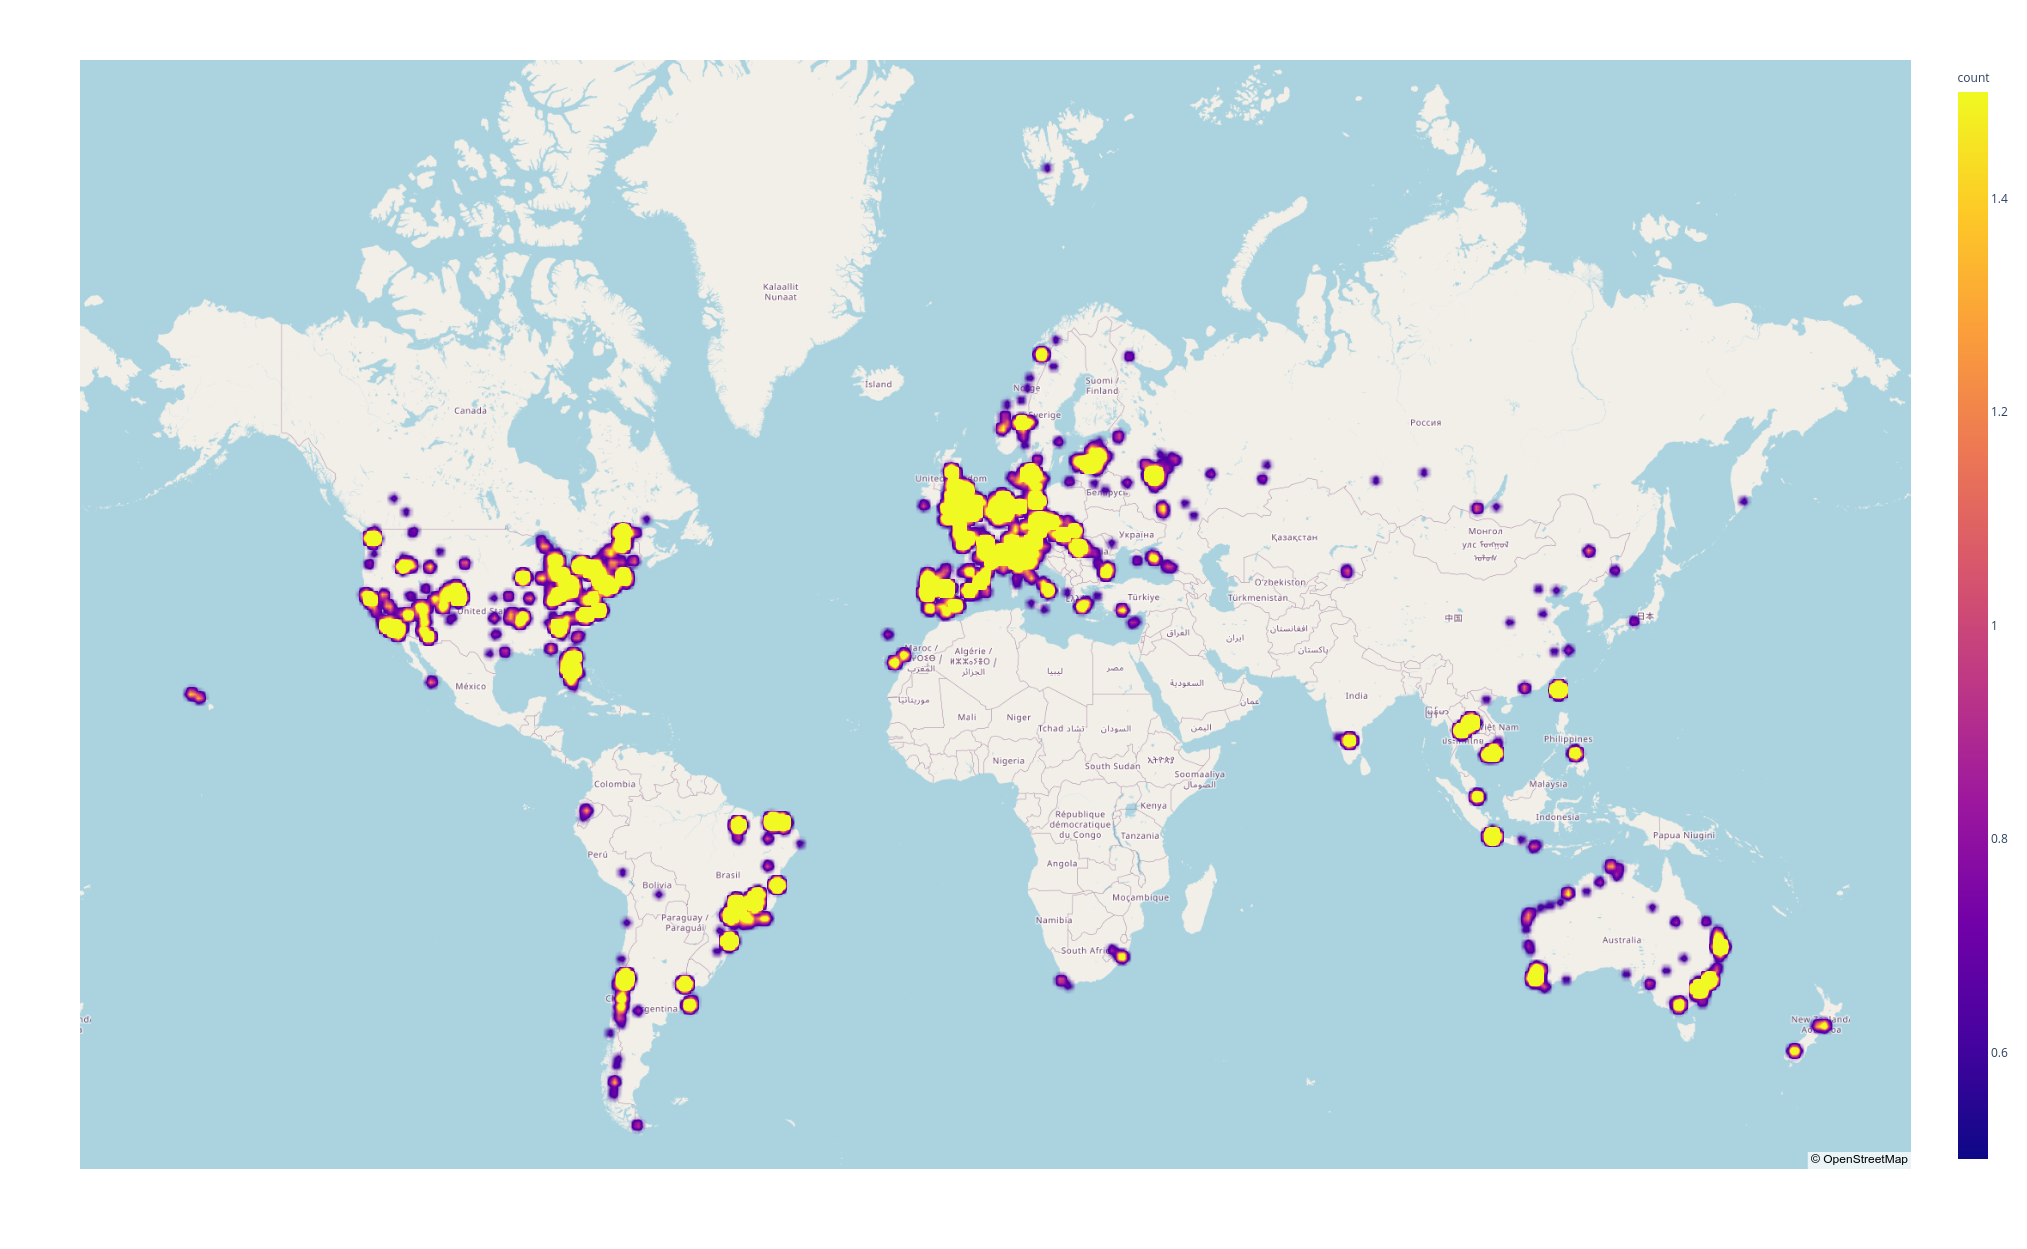
\includegraphics[width=\textwidth]{fig/Afwijkingen&Analyses/Heatmap.png}
    \caption{Geografische spreiding van de activiteiten in de dataset}\label{fig:geographic_spread}
\end{figure}
\begin{table}[h]
    \centering
    \begin{tabular}{|l||c|}
        \hline
        \textbf{Waarde}                       & \textbf{Aantal} \\
        \hline \hline
        Total number of users                 & 101             \\
        \hline
        Total number of activities            & 41 554          \\
        \hline
        Average \# activiteiten per user      & 411             \\
        \hline
        Median of \# activities per user      & 296             \\
        \hline
        Maximal \# activities for single user & 2946            \\
        \hline
        Minimal \# activities for single user & 31              \\
        \hline
    \end{tabular}
    \captionsetup{justification=centering}
    \caption{Overzicht van gebruikers en activiteiten}\label{tab:stats_dataset}
\end{table}
\begin{figure}[h]
    \centering
    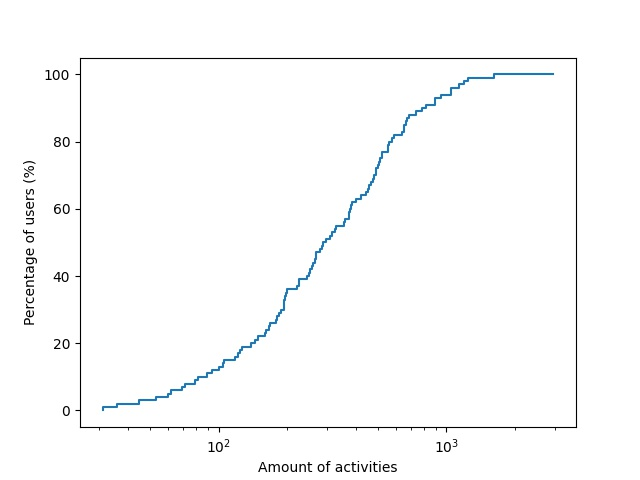
\includegraphics[width=0.9\textwidth]{fig/Afwijkingen&Analyses/CDF_amountActivities.jpg}
    \caption{\ac{CDF} plot van het aantal activiteiten per gebruiker}\label{fig:cdf_amount_activities}
\end{figure}

Let wel, alhoewel niet expliciet vermeld
door~\citeauthor{Dhondt_Pochat_Voulimeneas_Joosen_Volckaert_2022}, is er een
vermoeden dat er bewust gezocht werd naar gebruikers met een zo groot mogelijk
aantal activiteiten per gebruiker. Dit is een logische keuze, aangezien de
aanval een hogere kans op slagen heeft bij users die meer activiteiten hebben.
Wanneer we dit vergelijken met cijfers uit een studie die Strava zelf voerde in
2020, is er toch een mismatch terug te vinden~\cite{StravaMi72:online}. Het
persbericht, waarvan Figuur~\ref{fig:3billionUsers} is overgenomen, stelt dat
Strava in 2020 iets meer dan 50 miljoen gebruikers had, die samen in totaal
drie miljard activiteiten op het platform hebben geplaatst. Indien we deze
waarden omrekenen naar een gemiddelde, komen we uit op een ruwe geschatte 60
activiteiten per gebruiker ($\frac{3 \cdot 10^9}{5 \cdot 10^7} = 60 $). Dit is
een stuk lager dan de gemiddelde 411 activiteiten per gebruiker in de dataset.
De conclusies die dus getrokken worden uit deze steekproef mogen niet zomaar
veralgemeend worden naar de volledige gebruikersbasis van Strava.
\begin{figure}[H]
    \centering
    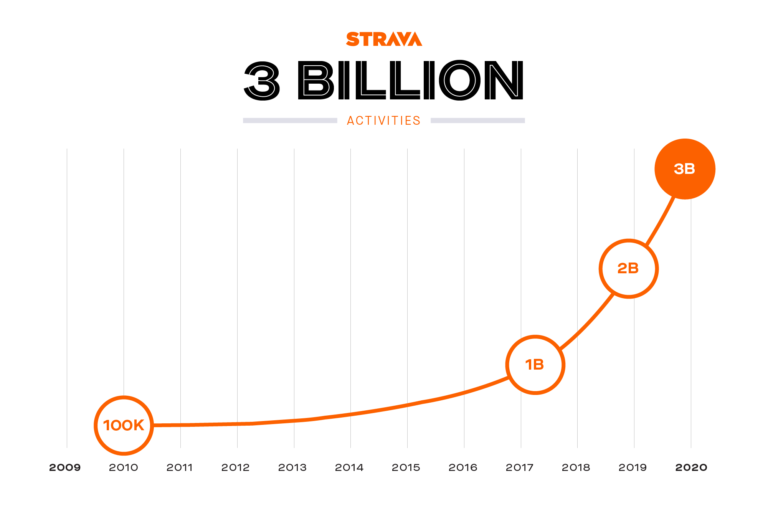
\includegraphics[width=0.5\textwidth]{fig/Strava_3billion.png}
    \caption{Post op sociale media van Strava die de evolutie van het totaal aantal activiteiten weergeeft~\cite{StravaMi72:online}}\label{fig:3billionUsers}
\end{figure}

\section{Mogelijke afwijkingen binnenin de dataset}
Doordat de dataset niet expliciet werd gecheckt op onnauwkeurigheden en een
willekeurige sample is, Doordat deze dataset niet door Strava zelf werd
vrijgegeven, maar manueel afgehaald werd via scraping, is er een grote kans op
activiteiten die afwijkingen of fouten vertonen. Zeker door het belang van
\ac{gps}-data, die een grote kans heeft op fouten, in deze studie is het
belangrijk om de dataset te analyseren op deze mogelijke afwijkingen. Gps-data
is een signaal die a.d.h.v.\ gekende locaties van satellieten, gecombineerd met
de tijd die het signaal nodig heeft om deze satellieten te bereiken, de locatie
van een gebruiker kan bepalen~\cite{BadGPSDa19:online}. Door de snelheid van
het signaal, kunnen kleine vertragingen in het signaal al een grote invloed
hebben op de accuraatheid van de data. Andere factoren zoals hoge bomen of
gebouwen, maar ook de aanwezigheid van wolken kunnen een impact hebben op het
signaal. Ook de frequentie waarmee locatie wordt bepaald, wat afhankelijk is
van het gebruikte toestel kan meespellen.

\subsection{Mogelijke fouten bij gps-data}
Zoals reeds aangehaald kunnen er bij het verzamelen van \ac{gps}-data
significante fouten optreden. Met \ac{gps}-fouten wordt gedoeld op data die de
\ac{gps}-sensor opvangt die niet overeenstemt met de werkelijke
\ac{gps}-locatie. Deze fouten kunnen verschillende oorzaken hebben. De
belangrijkste zijn hierbij \textit{\ac{gps}-drift}, \textit{\ac{gps}-signal
    loss} en \textit{\ac{gps}-bounce}.

Gps-drift is een fenomeen waarbij de \ac{gps}-locatie van een gebruiker afwijkt
van de effectieve locatie. Een voorbeeld vanuit het Strava-platform is terug te
vinden op Figuur~\ref{fig:gps_drift_Strava}. Hierbij is te zien dat de
gebruiker een deel van de route door gebouwen heen en door het water aflegt.
Dit kan worden veroorzaakt door dichtbebouwde omgevingen, en omgevingsfactoren
zoals hoge bomen. Om dit tegen te gaan, zou eventueel de eerder beschreven
methode van map-snapping kunnen worden toegepast.
\begin{figure}[h]
    \centering
    \begin{subfigure}[b]{.45\textwidth}
        \centering
        \includegraphics[width=\textwidth]{fig/Afwijkingen&Analyses/Crooked Routes/GPS-drift.png}
        \caption{Voorbeeld van gps-drift op Strava}\label{fig:gps_drift_Strava}
    \end{subfigure}\hfill
    \begin{subfigure}[b]{.49\textwidth}
        \centering
        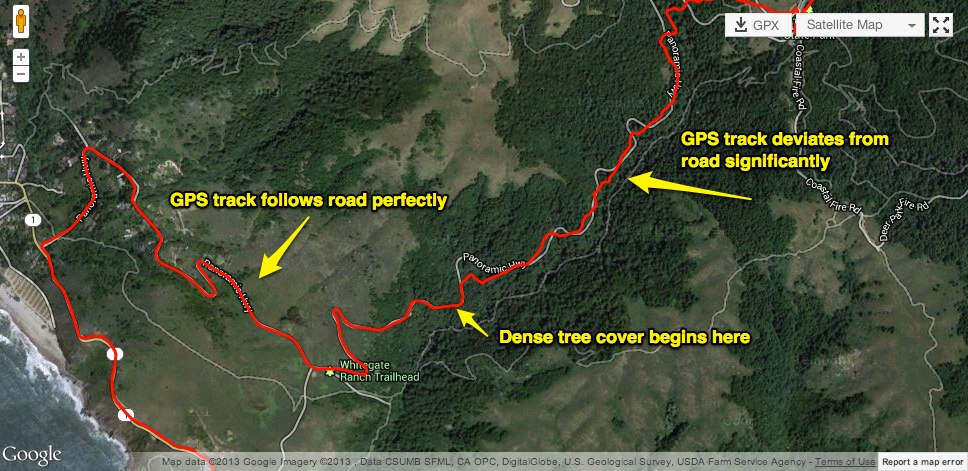
\includegraphics[width=\textwidth]{fig/Afwijkingen&Analyses/Crooked Routes/GPS-Drift_onlnie.jpg}
        \caption{Voorbeeld van gps-drift op een satellietkaart, veroorzaakt door dichte boomgroei~\cite{BadGPSDa19:online}}
    \end{subfigure}
    \caption{Voorbeelden van gps-drift}
\end{figure}

Gps-bouncing is een fenomeen veroorzaakt door hoge gebouwen. Het
\ac{gps}-signaal zal hierbij over en weer weerkaatsen tussen de gebouwen, op
weg naar de satelliet. Hierdoor verondersteld het apparaat afgelegde afstand
bij het berekenen van de locatie, door de extra vertraging. De uitkomst van het
traject is dan onvoorspelbaar, wat leidt tot een `cluster' van \ac{gps}-punten
wanneer dit voor een paar punten in dezelfde omgeving gebeurt. Voorbeelden
hiervan zijn terug te vinden op Figuur~\ref{fig:gps_bounce}. Om dit fenomeen op
zijn beurt tegen te gaan, is het best om smoothing te toe te passen bij het
berekenen.
\begin{figure}
    \centering
    \begin{subfigure}[b]{0.49\textwidth}
        \centering
        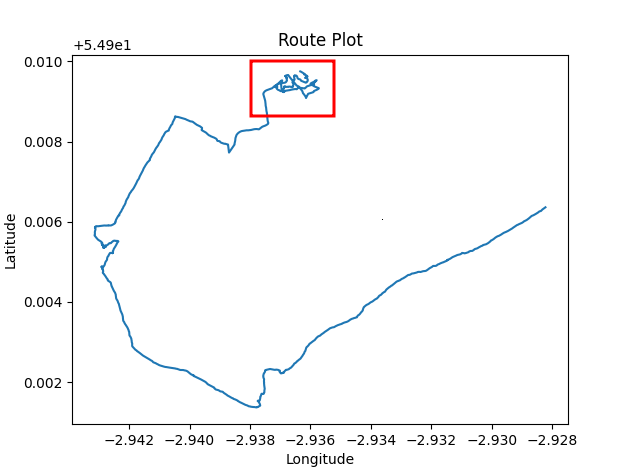
\includegraphics[width=\textwidth]{fig/Afwijkingen&Analyses/Crooked Routes/Crooked GPS Route_Cart.png}
    \end{subfigure}
    \begin{subfigure}[b]{0.49\textwidth}
        \centering
        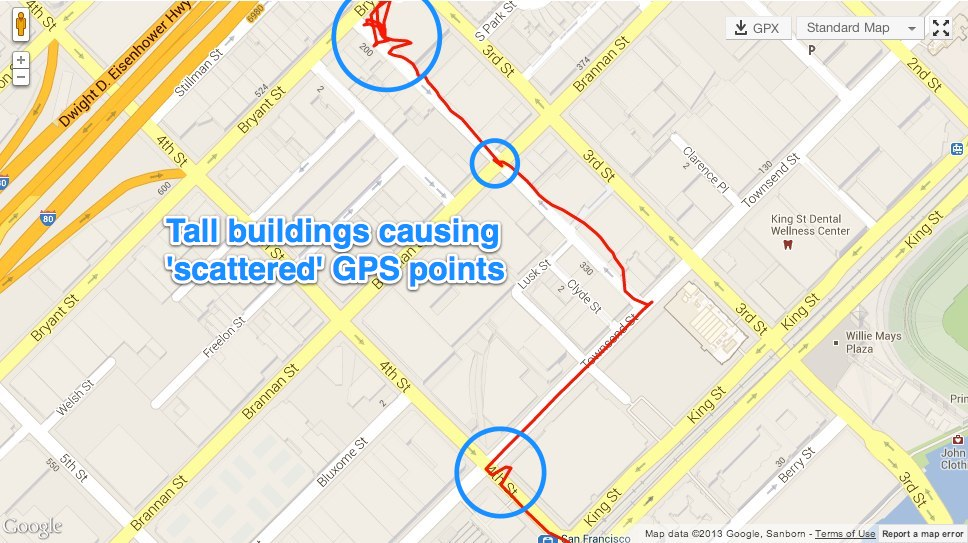
\includegraphics[width=\textwidth]{fig/Afwijkingen&Analyses/Crooked Routes/GPS_bounce_map.jpg}
    \end{subfigure}
    \caption{Voorbeelden van \ac{gps}-bounce~\cite{BadGPSDa19:online}}\label{fig:gps_bounce}
\end{figure}

Er zijn ook voorbeelden waarbij beide fenomenen voorkomen, zoals te zien is op
Figuur~\ref{fig:gps_drift_bounce_Strava}. Zoals te zien is op deze figuur, zal
indien op een intuïtieve manier de afstand wordt berekend (door gewoon het
afstandsverschil tussen twee opeenvolgende punten te nemen), een significant
verschil zijn tussen de afstand die de gebruiker werkelijk afgelegd heeft, en
de berekende afstand.
\begin{figure}
    \centering
    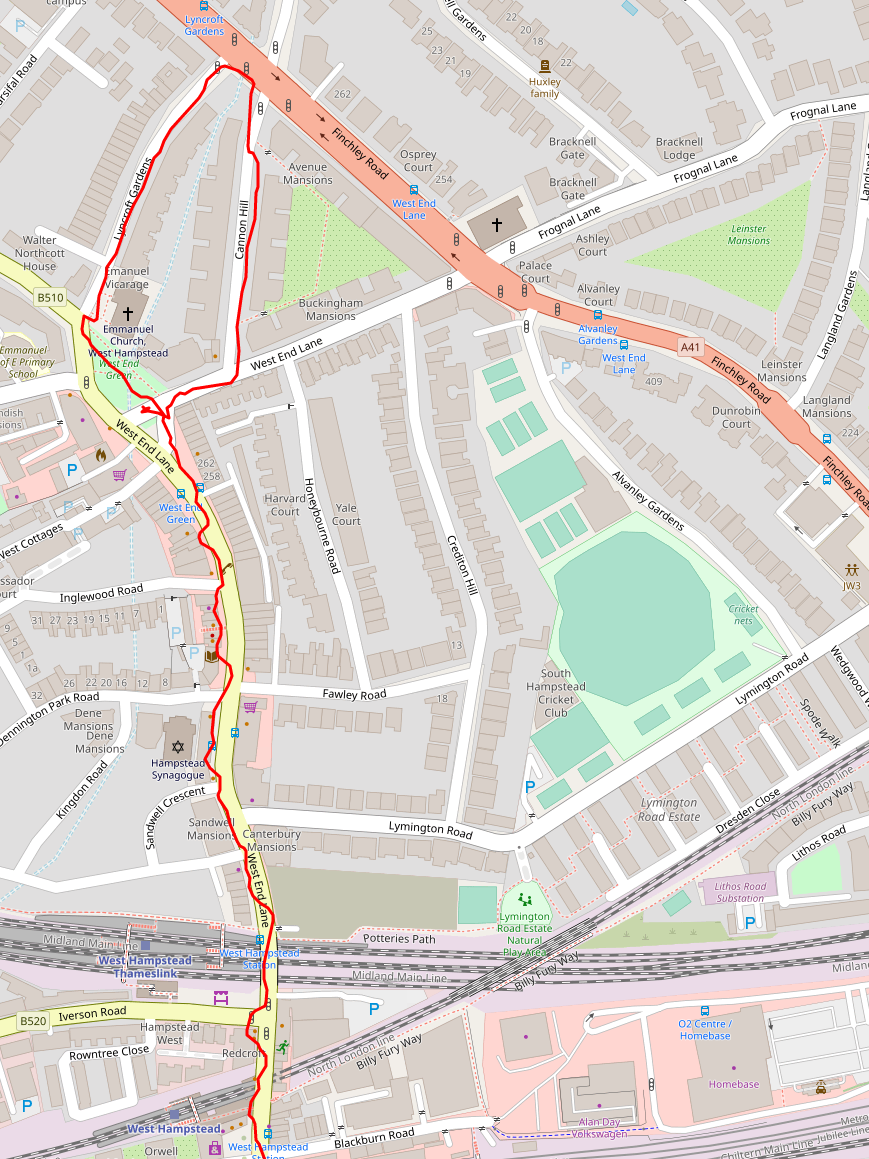
\includegraphics[width=0.7\textwidth]{fig/Afwijkingen&Analyses/Crooked Routes/1_notSnapped.png}
    \caption{Voorbeeld van zowel gps-drift en gps-bounce uit de gebruikte dataset}\label{fig:gps_drift_bounce_Strava}
\end{figure}

Een laatste fenomeen dat kan optreden is \ac{gps}-signal loss. Hierbij gaat het
signaal van de gebruiker verloren, en wordt pas op een later tijdstip terug een
nieuw signaal verzonden, waardoor een sprong werd gemaakt. In dit geval zou map
matching opnieuw een goede oplossing om dit te omzeilen. Een tweede oorzaak die
kan leiden tot signal loss, die zeker van toepassing is bij fitness trackers,
is de mogelijkheid tot het pauzeren van een activiteit. In dit geval wordt de
activiteit gepauzeerd voor een bepaald tijdsframe, en wordt er geen data meer
verzameld. Wanneer de activiteit terug wordt hervat, zal er een sprong zijn in
de \ac{gps}-locaties, wat kan leiden tot een verkeerde berekening van de
afstand. In het geval van een pauze zal mapmatching geen oplossing zijn, maar
zou deze `sprongafstand' best weggelaten worden in de berekeningen. Een
voorbeeld hiervan is terug te vinden op Figuur~\ref{fig:gps_signal_loss}.
\begin{figure}
    \begin{subfigure}[b]{0.49\textwidth}
        \centering
        \includegraphics[width=\textwidth]{fig/Afwijkingen&Analyses/Crooked Routes/1_Full_withArrow.png}
    \end{subfigure}
    \begin{subfigure}[b]{0.49\textwidth}
        \centering
        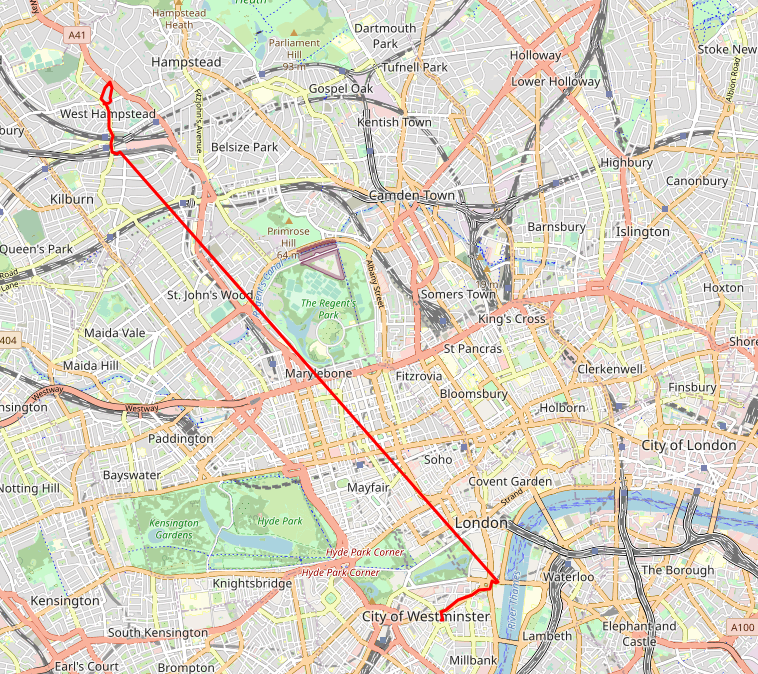
\includegraphics[width=\textwidth]{fig/Afwijkingen&Analyses/Crooked Routes/1_Full_original.png}
    \end{subfigure}
    \caption{Voorbeeld van signal loss uit de gebruikte dataset}\label{fig:gps_signal_loss}
\end{figure}

\subsection{Gps-fouten in de gebruikte dataset}
Allereerst onderzoeken we naar de aanwezigheid van \ac{gps}-fouten in de vorm
van signal losses of pauzes. Dit gebeurt door de afstand tussen twee
opeenvolgende \ac{gps}-punten te bestuderen.
Tabel~\ref{tab:distance_between_gps_points_table} geeft een globaal overzicht
van deze verdeling, en de volledige verdeling is terug te vinden op
Figuur~\ref{fig:distance_between_gps_points_CDF}. De gemiddelde afstand tussen
twee opeenvolgende locaties is $6.41m$, met een standaardafwijking van
$42.53m$. Het gemiddelde is relatief laag, wat kan wijzen op accurate gegevens,
maar de hoge standaardafwijking wijst op grote schommelingen. Op de grafiek en
de tabel is te zien dat de meeste afstanden onder de $20m$ liggen, wat opnieuw
een indicatie kan zijn van een degelijke precisie. Er is echter wel een klein
deel van de \ac{gps}-punten die een grote onderlinge afstanden vertoond. Door
de omvang van het aantal \ac{gps}-punten, en een gemiddeld aantal punten per
activiteit van $2574.90$, valt dit zeker niet te verwaarlozen. Als we empirisch
stellen dat een significant verschil $50m$ bedraagt, dan ligt 0.9\% van de data
boven deze drempel. Per activiteit zou dit dan resulteren op gemiddeld $23$
afwijkende punten, wat zeker kan zorgen voor een significante afwijking op de
resulterende afstand.
\begin{table}[h]
    \centering
    \begin{tabular}{lr}
        \toprule
        \midrule
        Total number of gps-points              & $1.070 \cdot 10^8$        \\
        \hline
        distance between 2 gps points $>$ 10m   & $13.91\%$                 \\
        distance between 2 gps points $>$ 20m   & $5.44\%$                  \\
        distance between 2 gps points $>$ 50m   & $9.02 \cdot 10^{-1}\%$    \\
        distance between 2 gps points $>$ 75m   & $2.21 \cdot 10^{-2}\%$    \\
        distance between 2 gps points $>$ 100m  & $1.30 \cdot 10^{-2}\%$    \\
        distance between 2 gps points $>$ 150m  & $8.04 \cdot 10^{-3}\%$    \\
        distance between 2 gps points $>$ 200m  & $6.071 \cdot  10^{-3} \%$ \\
        distance between 2 gps points $>$ 500m  & $2.600 \cdot 10^{-3} \%$  \\
        distance between 2 gps points $>$ 1000m & $1.345 \cdot 10^{-3}$ \%  \\
        distance between 2 gps points $>$ 2000m & $4.056 \cdot 10^{-4} \%$  \\
        \midrule
        \bottomrule
    \end{tabular}
    \captionsetup{justification=centering}
    \caption{Verdeling van de afstanden tussen twee opeenvolgende gps-punten}\label{tab:distance_between_gps_points_table}
\end{table}
\begin{figure}
    \centering
    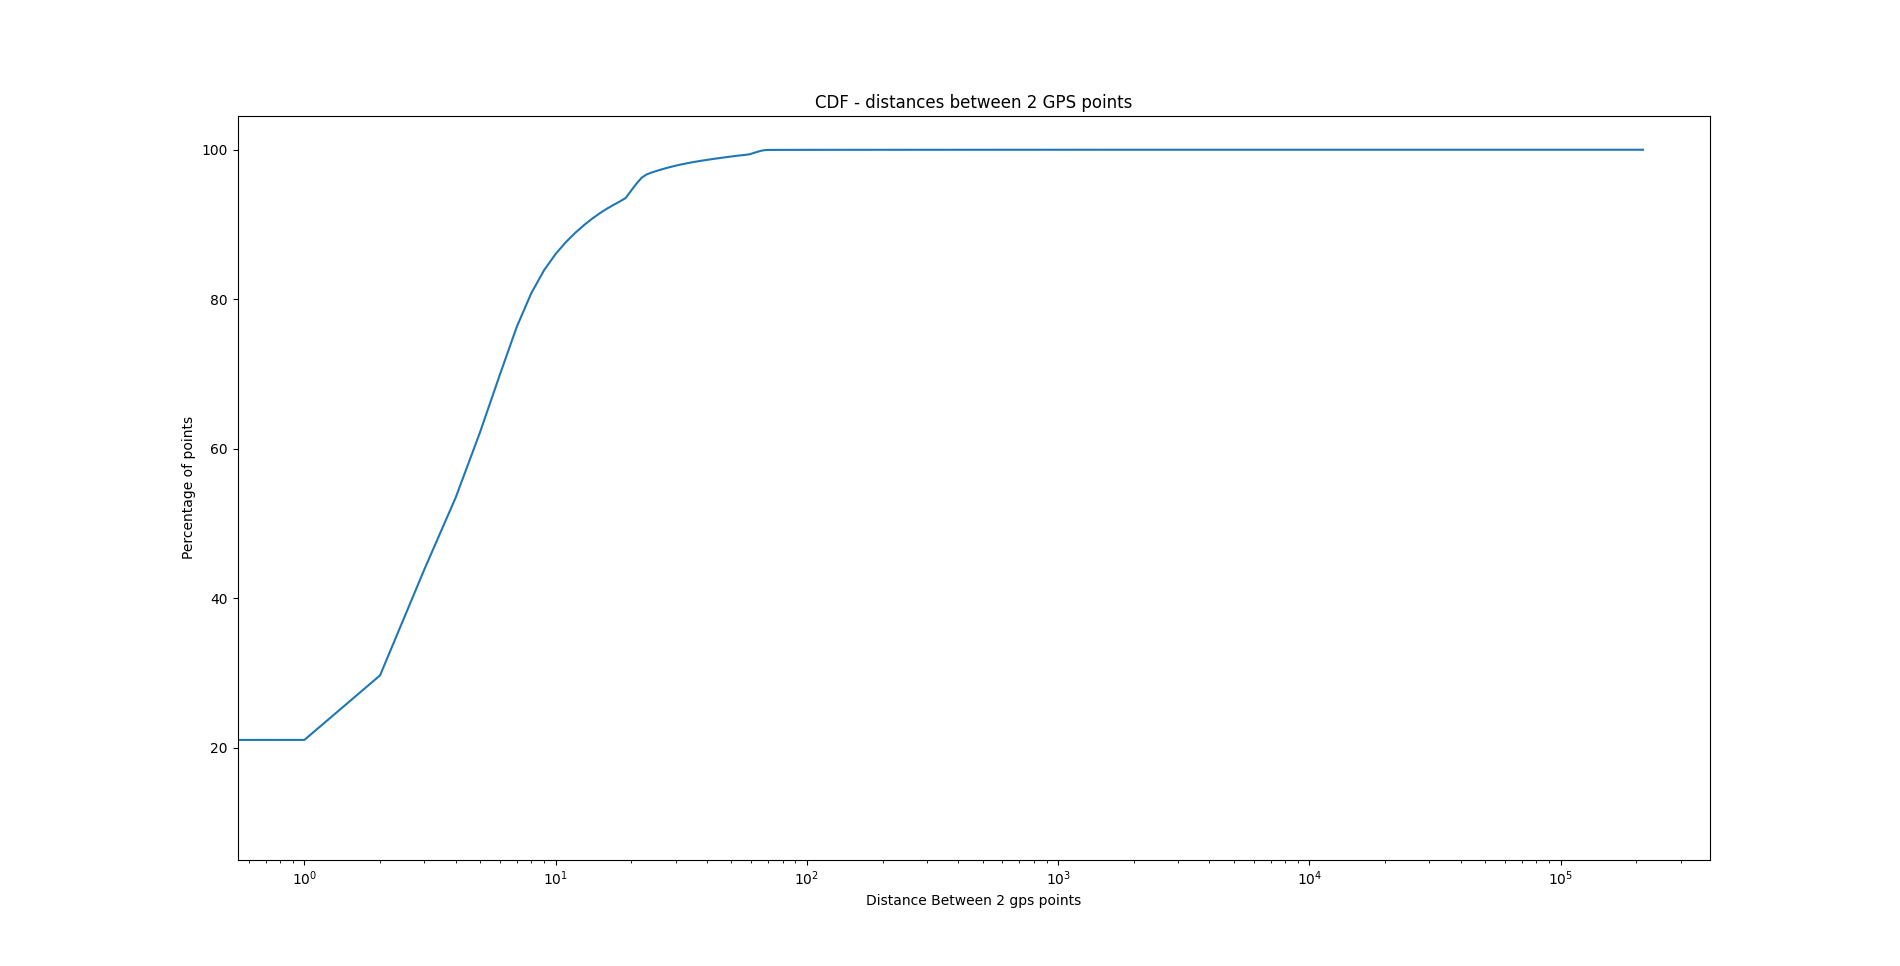
\includegraphics[width=\textwidth]{fig/Afwijkingen&Analyses/Graphs/Afstand tussen 2 gps-punten.png}
    \caption{Verdeling van de afstanden tussen twee opeenvolgende gps-punten}\label{fig:distance_between_gps_points_CDF}
\end{figure}

Om het aantal \ac{gps}-afwijkingen in de dataset te bepalen die relevant zijn
voor de aanval, wordt ook het verschil onderzocht tussen de berekende afstand
afgelegd buiten de \ac{EPZ} (het zichtbare traject) en de theoretisch afgelegde
afstand buiten de \ac{EPZ}, die af te lezen valt uit de dataset via de
cumulatieve afstand\footnote{Er wordt gesproken van een theoretische waarde,
    maar deze is eigenlijk de berekende waarde volgens het platform. We beschouwen
    deze dus als referentie.}. Een eerste visualisatie is te zien op
Figuur~\ref{fig:difference_noCDF}. De figuur illustreert de schommelingen
tussen de handmatig berekende afstand en de theoretische afstand van één
gebruiker. De pieken duiden op duidelijk sterk afwijkende berekende afstanden,
en dus ook op grote \ac{gps}-fouten. Maar ook de schommelingen die iets minder
opvallend zijn duiden op grote inaccuraatheden tussen de berekende en
theoretische afstanden. Voor de volledige dataset wordt gebruik gemaakt van
\ac{CDF}-plots. De resultaten worden weergegeven op
Figuur~\ref{fig:differences_theoretical}. Figuur~\ref{fig:differences_log}
bevat de verdeling voor alle activiteiten, gebruik makend van een logaritmische
schaal. Figuur~\ref{fig:differences_nolog} toont 95\% van de activiteiten met
de kleinste verschillen, om een beter beeld te krijgen van de grootte van de
meeste verschillen. Op de grafieken valt op dat heel wat significante
verschillen aanwezig zijn. Dit duidt op het relatief zwaar doorwegen van de
\ac{gps}-fouten in de dataset. Aangezien het gaat over bepalen van woonplaatsen
of andere gevoelige locaties, kunnen afwijkingen vanaf 50 à 100 meter al
relevant zijn. Daarnaast gaat het vaak over kleine afwijkingen op een heel wat
punten, wat kan resulteren in een grote afwijking. De grafieken tonen aan dat
er bij de ruwe ontvangen data heel wat \ac{gps}-fouten aanwezig zijn. Smoothing
zal dus zeker nodig zijn om deze te beperken.

\begin{figure}
    \centering
    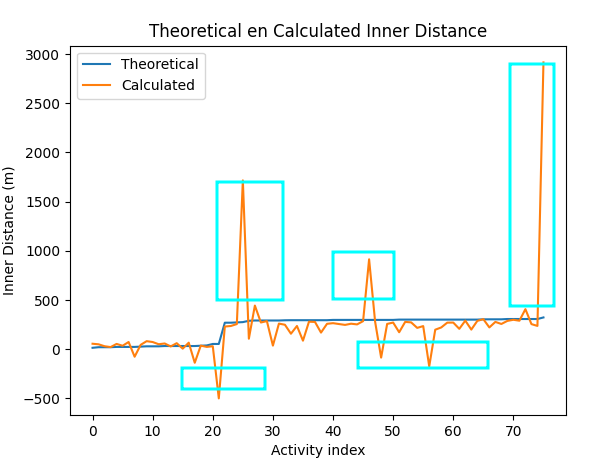
\includegraphics[width=\textwidth]{fig/Afwijkingen&Analyses/Graphs/Verschil_Theoretische_innerDistance.png}
    \caption{Verschil tussen de berekende afstand en de theoretische afstand voor één gebruiker}\label{fig:difference_noCDF}
\end{figure}
\begin{figure}[h]
    \centering
    \begin{subfigure}{0.85\textwidth}
        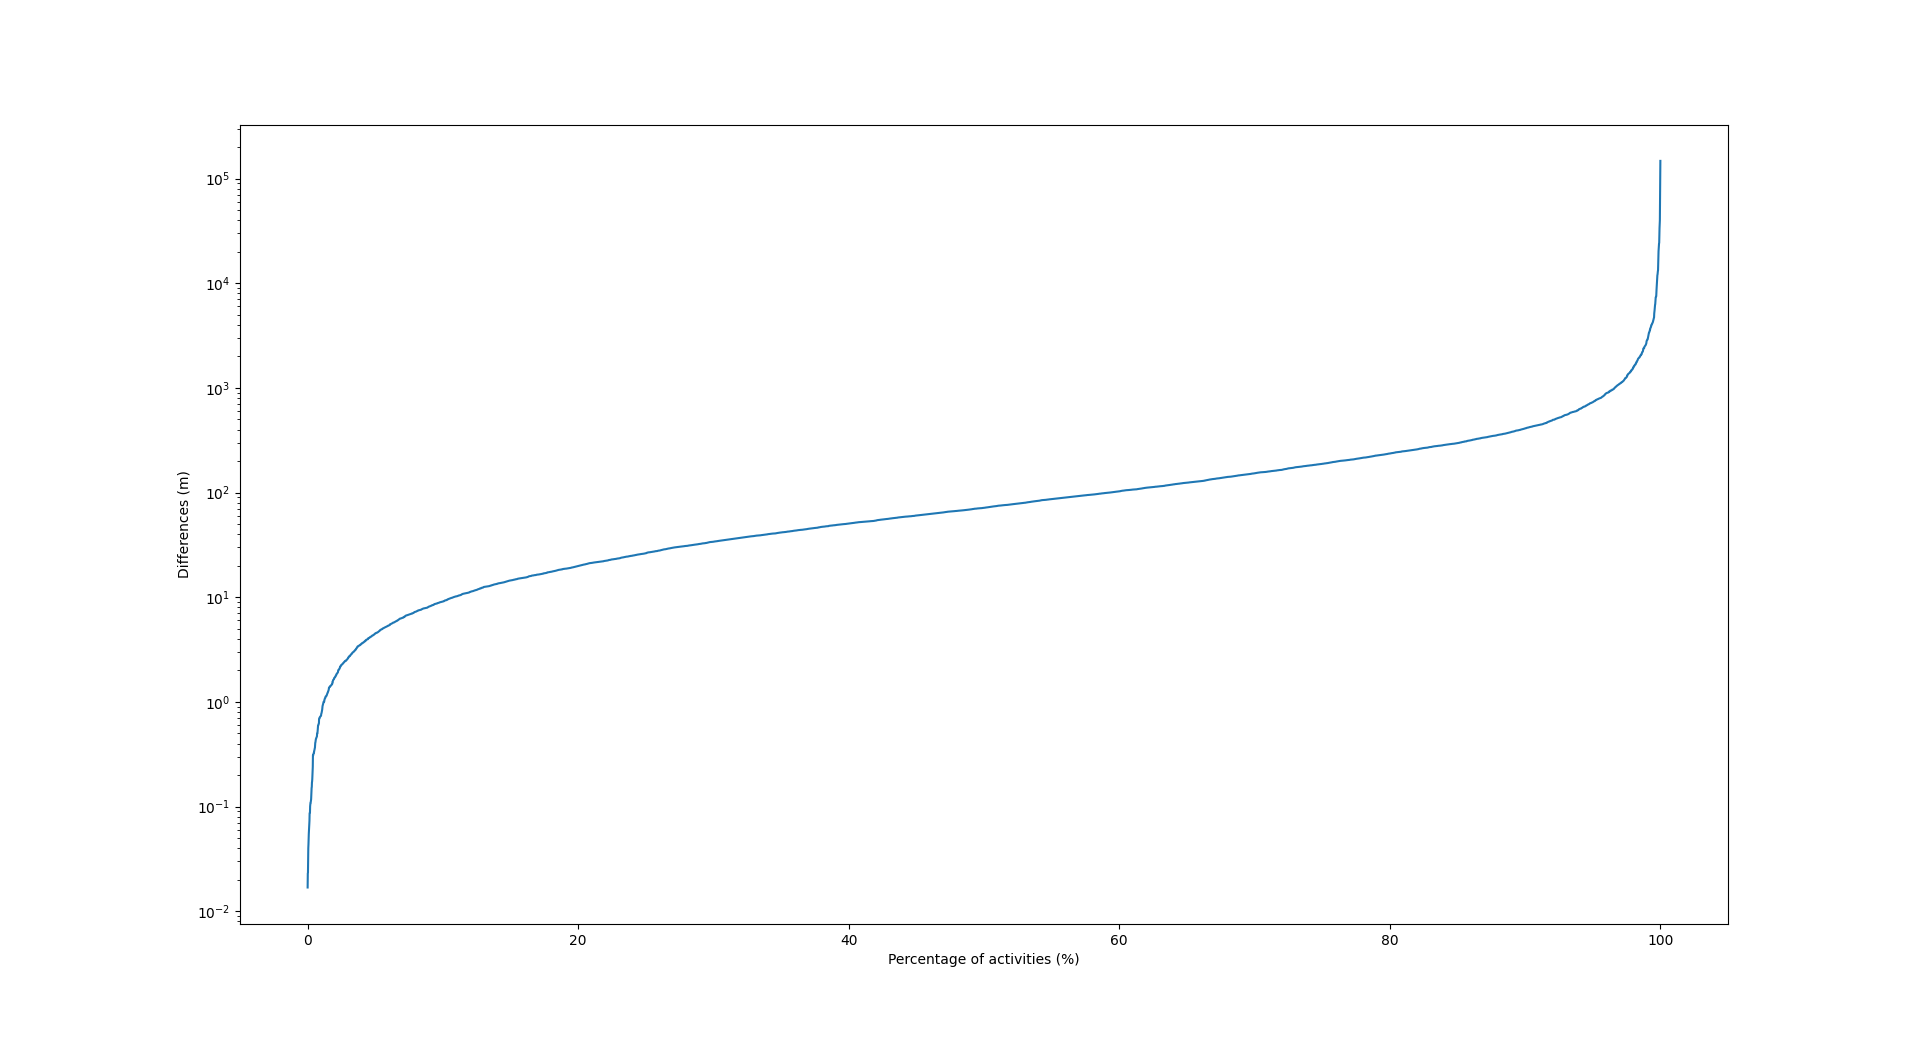
\includegraphics[width=\textwidth]{fig/Afwijkingen&Analyses/Graphs/100_Differences_tov_theoretische_BefSmoothening.png}
        \caption{100\% van de activiteiten (logaritmische schaal)}\label{fig:differences_log}
    \end{subfigure}
    \begin{subfigure}[b]{0.85\textwidth}
        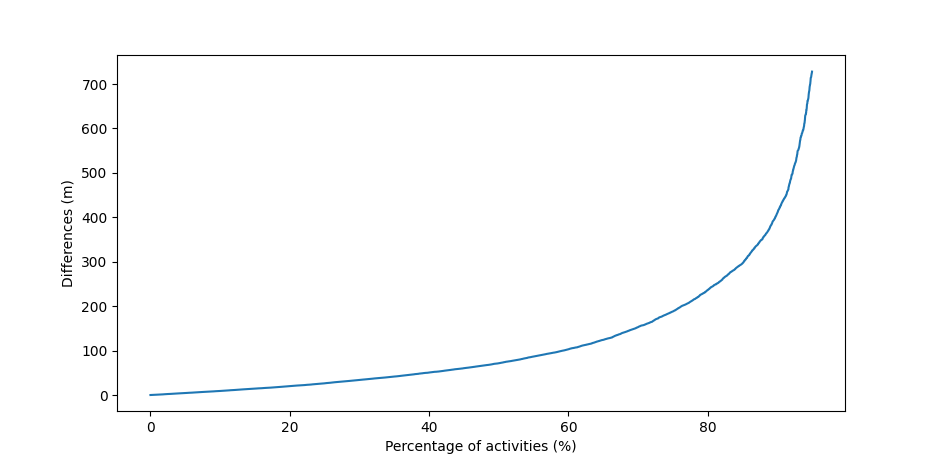
\includegraphics[width=\textwidth]{fig/Afwijkingen&Analyses/Graphs/95_Differences_tov_theoretische_BefSmoothening.png}
        \caption{95\% van de activiteiten}\label{fig:differences_nolog}m
    \end{subfigure}
    \caption{Verdeling van het verschil tussen de berekende afstand en de theoretische afstand buiten de \ac{EPZ} }\label{fig:differences_theoretical}
\end{figure}

\section{Technieken gps-data te verbeteren}
Om de accuraatheid van de \ac{gps}-data te verbeteren, en zo een betere
\textit{outer distance} te kunnen berekenen en uiteindelijk een accuratere
aanval te bekomen, worden enkele technieken toegepast. Zoals besproken in
Sectie~\ref{sec:afstandsberekeningen_strava} is de hypothese dat de
fitness-platformen gebruik maken van technieken om de \ac{gps}-data te
verbeteren. De besproken technieken waren \textit{map matching} en
\textit{\ac{gps}-smoothing}. Bij de uitvoering van de aanvallen wordt smoothing
toegepast. Er wordt dan ook geëxperimenteerd met verschillende smoothing
windows, op zoek naar het window met het beste effect op de aanval.

Daarnaast passen we ook een filtering toe die rekening houdt met
\ac{gps}-sprongen. Het idee is te stellen dat wanneer \ac{gps}-sprongen
gebeuren, en er dus een te grote afstand tussen twee opeenvolgende punten is
deze afstand niet te laten meetellen. Dit is echter wel niet vanzelfsprekend,
aangezien dit wel kan worden meeberekent door de platformen. Stel dat wij een
sprong van $50m$ laten vallen, maar de platformen laten deze wel meetellen, dan
zullen we de afwijking op het eindresultaat enkel maar verhogen. Het drempel
voor de filtering moet dus hoog genoeg zijn om deze voorvallen te vermijden. In
dit onderzoek kozen we voor een drempelwaarde van $200m$.

% EXTRAAAA
% \section{Stilstaande gebruiker}
% In Sectie~\ref{sec:definitie-aanvaller} wordt de aanvaller assumptie gemaakt
% dat een gebruiker niet mag stilstaan binnen de~\ac{EPZ}. Deze is enkel van
% toepassing indien de berekening gebeurt op basis van de totale verstreken tijd. Op Figuur~\ref{fig:time_diff} zien we dat de verschillen
%%%%%%%%%%%%%%%%%%%%%%%%%%%%%%%%%%%%%%%%%%%%%%%%%%%%%%%%%%%%%%%%%%% 
%                                                                 %
%                            CHAPTER                              %
%                                                                 %
%%%%%%%%%%%%%%%%%%%%%%%%%%%%%%%%%%%%%%%%%%%%%%%%%%%%%%%%%%%%%%%%%%% 
\chapter{Conclusies}

% Bibliografie: referenties. De items zitten in bibliografie.bib
%%%%%%%%%%%%%%%%%%%%%%%%%%%%%%%%%%%%%%%%%%%%%%%%%%%%%%%%%%%%%%%%%
% Indien je ook de niet geciteerde werken in je bibliografie wil opnemen, commentarieer dan onderstaande regel uit!
\nocite{*}
\bibliographystyle{apalike} % Gebruik ieeetr voor nummers
\bibliography{bibliografie}

% Eventueel enkele appendices
%%%%%%%%%%%%%%%%%%%%%%%%%%%%%%
\appendix
\chapter{Uitleg over de appendices}
Bijlagen worden bij voorkeur enkel elektronisch ter beschikking gesteld. Indien essentieel kunnen in overleg met de promotor bijlagen in de scriptie opgenomen worden of als apart boekdeel voorzien worden.

Er wordt wel steeds een lijst met vermelding van alle bijlagen opgenomen in de scriptie. Bijlagen worden genummerd het een drukletter A, B, C,...

Voorbeelden van bijlagen:\\
Bijlage A: \qquad	Detailtekeningen van de proefopstelling \\
Bijlage B: \qquad	Meetgegevens (op USB)
\\






\includepdf{private/back_fiiw_gent.pdf}
\end{document}